
\documentclass[11pt]{article}
\usepackage[T1]{fontenc}
\usepackage[utf8]{inputenc}
\usepackage[margin=0.86in]{geometry}
\usepackage{amsmath,amssymb,amsfonts,amsthm,mathtools}
\usepackage{booktabs,longtable,array,enumitem,graphicx,xcolor,hyperref,cleveref}
\usepackage{listings}
\usepackage{tikz}
\usetikzlibrary{arrows.meta,positioning,shapes.geometric,fit,calc,decorations.pathmorphing}
\hypersetup{colorlinks=true,linkcolor=blue!50!black,citecolor=blue!50!black,urlcolor=blue!50!black}
\definecolor{darkblue}{RGB}{25,76,130}
\definecolor{darkgreen}{RGB}{20,105,70}
\definecolor{darkred}{RGB}{130,40,40}
\definecolor{darkorange}{RGB}{170,90,20}
\definecolor{softgray}{RGB}{246,247,250}
\definecolor{softblue}{RGB}{235,243,252}
\definecolor{softgreen}{RGB}{235,249,240}
\definecolor{softorange}{RGB}{255,246,232}
\definecolor{softred}{RGB}{253,238,238}
\newtheorem{definition}{Definition}[section]
\newtheorem{assumption}[definition]{Assumption}
\newtheorem{theorem}[definition]{Theorem}
\newtheorem{proposition}[definition]{Proposition}
\newtheorem{lemma}[definition]{Lemma}
\newtheorem{corollary}[definition]{Corollary}
\newtheorem{example}[definition]{Example}
\newtheorem{remark}[definition]{Remark}
\newcommand{\R}{\mathbb{R}}
\newcommand{\N}{\mathbb{N}}
\newcommand{\Z}{\mathbb{Z}}
\newcommand{\Q}{\mathbb{Q}}
\newcommand{\T}{\mathbb{T}}
\newcommand{\K}{\mathbb{K}}
\newcommand{\E}{\mathbb{E}}
\newcommand{\Prob}{\mathbb{P}}
\newcommand{\calA}{\mathcal{A}}
\newcommand{\calB}{\mathcal{B}}
\newcommand{\calC}{\mathcal{C}}
\newcommand{\calD}{\mathcal{D}}
\newcommand{\calE}{\mathcal{E}}
\newcommand{\calF}{\mathcal{F}}
\newcommand{\calG}{\mathcal{G}}
\newcommand{\calH}{\mathcal{H}}
\newcommand{\calI}{\mathcal{I}}
\newcommand{\calK}{\mathcal{K}}
\newcommand{\calL}{\mathcal{L}}
\newcommand{\calM}{\mathcal{M}}
\newcommand{\calN}{\mathcal{N}}
\newcommand{\calO}{\mathcal{O}}
\newcommand{\calP}{\mathcal{P}}
\newcommand{\calQ}{\mathcal{Q}}
\newcommand{\calR}{\mathcal{R}}
\newcommand{\calS}{\mathcal{S}}
\newcommand{\calT}{\mathcal{T}}
\newcommand{\calU}{\mathcal{U}}
\newcommand{\calV}{\mathcal{V}}
\newcommand{\calW}{\mathcal{W}}
\newcommand{\calX}{\mathcal{X}}
\newcommand{\calY}{\mathcal{Y}}
\newcommand{\calZ}{\mathcal{Z}}
\newcommand{\oplusT}{\oplus_{\rm trop}}
\newcommand{\odotT}{\odot_{\rm trop}}
\newcommand{\argmax}{\operatorname*{arg\,max}}
\newcommand{\argmin}{\operatorname*{arg\,min}}
\newcommand{\softmax}{\operatorname{softmax}}
\newcommand{\LSE}{\operatorname{LSE}}
\newcommand{\diag}{\operatorname{diag}}
\newcommand{\dist}{\operatorname{dist}}
\newcommand{\rank}{\operatorname{rank}}
\newcommand{\Span}{\operatorname{span}}
\newcommand{\Conv}{\operatorname{Conv}}
\newcommand{\Val}{\operatorname{Val}}
\newcommand{\Log}{\operatorname{Log}}
\newcommand{\Trop}{\operatorname{Trop}}
\newcommand{\Hom}{\operatorname{Hom}}
\newcommand{\End}{\operatorname{End}}
\newcommand{\supp}{\operatorname{supp}}
\newcommand{\im}{\operatorname{im}}
\newcommand{\kerop}{\operatorname{ker}}
\newcommand{\bpb}{\operatorname{bits\mbox{-}per\mbox{-}byte}}
\newcommand{\norm}[1]{\left\lVert #1\right\rVert}
\newcommand{\abs}[1]{\left\lvert #1\right\rvert}
\newcommand{\ip}[2]{\left\langle #1,#2\right\rangle}
\newcommand{\trans}{^{\mathsf T}}
\newcommand{\eps}{\varepsilon}
\lstset{basicstyle=\ttfamily\small,breaklines=true,columns=fullflexible,frame=single,backgroundcolor=\color{softgray}}
\setlist[itemize]{leftmargin=1.25em,itemsep=2pt,topsep=2pt}
\setlist[enumerate]{leftmargin=1.4em,itemsep=2pt,topsep=2pt}
\sloppy

\title{\vspace{-1.4em}\textbf{TropicalGT II: Tropical Algebraic Geometry, Patchworked Reasoning Dynamics, and Persistent Polyhedral Training for Graph-Token Agents}}
\author{Amelie Schreiber}
\date{June 2026}

\begin{document}
\maketitle

\begin{abstract}
TropicalGT introduced a graph-token reasoning architecture whose attention core can operate in the max-plus or min-plus semiring, exposing active supports, polyhedral margins, and dynamic-programming certificates while preserving the bits-per-byte deployment discipline of the broader ToricGT program.  This paper develops the second iteration.  The guiding question is what tropical attention becomes when reasoning is not a single feed-forward pass but an iterative trajectory: a sequence of standardized reasoning steps, each with graph structure, hidden embeddings, retrieved evidence, verifier fields, filtered simplicial complexes, persistence summaries, tool records, and behavior controls.  We use tropical algebraic geometry to turn such trajectories into piecewise-linear and non-Archimedean objects: tropicalized reasoning amoebas, Newton subdivisions of proof alternatives, balanced tropical cycles of evidence flow, patchworked local reasoning charts, persistent tropical sufficient statistics, and ergodic cell-occupation summaries under repeated graph-to-graph updates.

The mathematical input comes from the same sources that make tropical algebraic geometry useful in classical enumerative geometry: amoebas and their logarithmic limits, non-Archimedean valuations, Kapranov-type hypersurface tropicalization, tropical curves with integer affine structure and balancing, Viro patchworking, Newton polygon subdivisions, correspondence theorems, and multiplicity formulas.  The modeling output is a training theory for reasoning agents.  A reasoning step is represented by a padded graph-token packet; a trajectory is a one-parameter family of such packets; its tropicalization is the finite polyhedral complex traced by active max-plus alternatives and valued embeddings.  We prove stability, equivariance, gluing, balancing, and ergodic statements under explicit finite or compact assumptions.  We then turn these statements into concrete objectives: tropical trajectory amoeba loss, patchworking gluing loss, cycle-balance residuals, valuation consistency, Newton-subdivision entropy, persistence-barcode tropical sufficient statistics, tropical Hilbert contraction, local-to-global evidence sheaf loss, ergodic occupation calibration, and bits-per-byte-gated certificate distillation.

The paper is written as a NeurIPS-style research-program article.  Theorems and proofs separate formal guarantees from empirical hypotheses.  Implementation sections give pseudocode, data schemas, exact audit routines, differentiable surrogates, and ablation protocols.  The practical message is direct: tropical mathematics should improve reasoning models only when it yields stable hidden algorithms, better long-context control, stronger out-of-distribution reasoning, lower artifact cost, or improved held-out bits-per-byte.  Otherwise it remains teacher-side diagnostic structure.
\end{abstract}

\tableofcontents
\newpage

\section{Introduction: from TropicalGT I to dynamical tropical reasoning}

TropicalGT I was motivated by a precise mismatch.  Many reasoning problems have sharp polyhedral structure.  Shortest paths, edit distance, Viterbi decoding, knapsack, subset sum, transitive closure, dynamic programming over graphs, and many proof-search relaxations are built from maximization or minimization plus ordinary addition.  Softmax attention can approximate these choices, but its normalization mixes all alternatives and its entropy can grow with length.  Tropical attention replaces a smooth mixture by an idempotent aggregation in the max-plus or min-plus semiring.  The NeurIPS 2025 Tropical Attention paper formalizes this perspective: multi-head tropical attention operates in tropical projective space, uses tropical Hilbert geometry, preserves piecewise-linear decision structure, and can approximate tropical circuits and transitive closure with polynomial resource bounds \cite{hashemi2025tropical,hashemi2025openreview}.  The released implementation exposes a standalone tropical attention kernel and experiments over graph and combinatorial algorithmic tasks such as Floyd-Warshall, Quickselect, subset sum, knapsack, strongly connected components, bin packing, and coin change \cite{hashemi2025code}.

TropicalGT I imported that kernel into a graph-token reasoning agent.  Its unit of computation was a typed graph token: a node, edge, tool call, memory record, retrieved chunk, proof obligation, or behavior label.  A tropical head computed
\begin{equation}
Y_{ic}=\max_j\{S_{ij}+V_{jc}\},
\end{equation}
while retaining the active support
\begin{equation}
A_{ic}=\argmax_j\{S_{ij}+V_{jc}\}
\end{equation}
and the top-two margin.  Active supports became finite certificates.  Large margins implied stable choices.  Blockwise max-plus scans gave exact long-context execution because maximum is associative and commutative.  The deployment rule was strict: auxiliary structure survives only if it improves held-out \(\bpb\), accuracy, retrieval, control, or some other predeclared metric after artifact-byte accounting.

This second paper extends the theory to the setting analogous to the second paper of the original ToricGT series.  Instead of studying one reasoning step in isolation, we study reasoning trajectories.  A model repeatedly applies a learned graph-to-graph map
\begin{equation}
F_\theta:R_t\longmapsto R_{t+1},
\end{equation}
where \(R_t\) is a standardized reasoning packet.  Each packet may include a partial answer, a graph-of-thought state, retrieved evidence, hidden embeddings, tool outputs, verifier scores, behavior coordinates, and a filtered simplicial complex built from the step.  Iterations fill a reasoning trajectory until the model has enough context to answer.  The central object is no longer a tropical attention head, but the dynamical system of tropicalized reasoning objects.

The tropical algebraic geometry book by Itenberg, Mikhalkin, and Shustin supplies the conceptual bridge.  It starts from amoebas of complex varieties, studies limits of logarithmically rescaled amoebas, introduces non-Archimedean amoebas and the tropical semifield, and treats tropical curves as metric graphs with integer affine structure \cite{itenberg2009}.  It then develops patchworking, showing how algebraic varieties can be glued from local pieces controlled by polyhedral subdivisions.  For enumerative geometry, tropicalization and patchworking become inverse operations: tropical curves and their local algebraic data can count or reconstruct classical curves in toric surfaces.  This paper imports that logic into model training.  A reasoning trajectory is a family of hidden algebraic-combinatorial objects; tropicalization extracts its finite piecewise-linear skeleton; patchworking glues local reasoning charts into a global answer; balancing expresses conservation of evidence and proof obligations; multiplicities express how many hidden completions support a visible answer; ergodic summaries describe repeated update dynamics over active cells.

\paragraph{The main thesis.}
Tropical algebraic geometry gives a language for turning hidden reasoning into finite, auditable, composable structure.  The language is useful for training only when it produces deployable gains.  Therefore every object in this paper is paired with: (i) a finite certificate, (ii) a differentiable surrogate, (iii) an exact or high-precision audit, (iv) a bits-per-byte or reasoning metric, and (v) an ablation gate.

\paragraph{Contributions.}
We make the following contributions.
\begin{enumerate}
\item We define \emph{tropical reasoning packets}, \emph{trajectory amoebas}, \emph{tropicalized graph-to-graph dynamics}, and \emph{tropical persistent reasoning modules}.
\item We adapt amoebas, non-Archimedean valuations, tropical polynomials, Newton subdivisions, balancing, patchworking, and correspondence-style multiplicities to iterative reasoning trajectories.
\item We prove stability, equivariance, gluing, conservation, persistence, and ergodic theorems under finite or compact assumptions.  These theorems do not claim that a neural network literally is an algebraic variety; they show that finite tropical certificates are well-defined and useful under explicit constructions.
\item We give a catalogue of training losses, metrics, objectives, and regularizers for dynamical tropical reasoning: patchworking losses, balancing residuals, valuation-consistency losses, cycle-handle penalties, tropical Hilbert contraction, persistent barcode losses, ergodic cell calibration, tropical correspondence multiplicity weighting, and bits-per-byte-gated distillation.
\item We provide implementation details for PyTorch/JAX-style models, including data schemas, pseudocode, audit procedures, approximation schedules, reproducibility criteria, and recommended ablations.
\end{enumerate}

\begin{figure}[t]
\centering
\resizebox{\textwidth}{!}{%
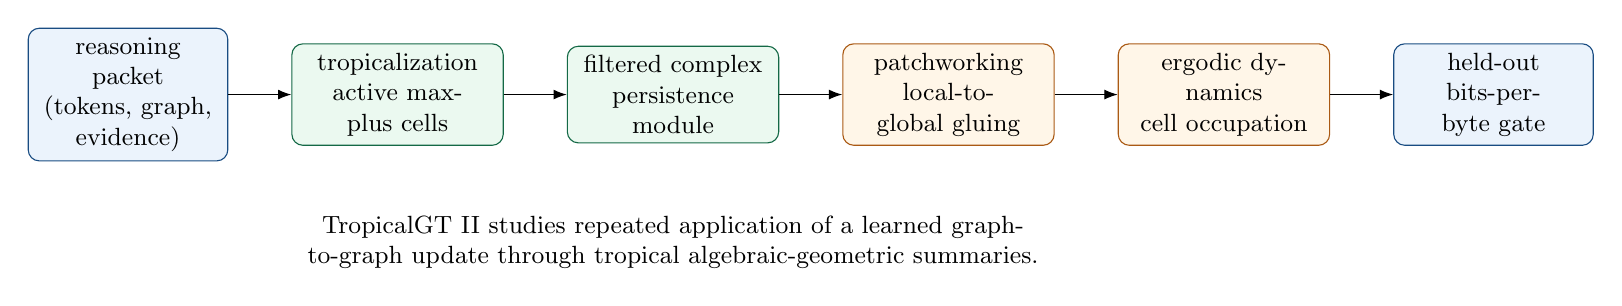
\begin{tikzpicture}[node distance=0.8cm,>=Latex, every node/.style={font=\small}]
\tikzstyle{box}=[rounded corners, draw=darkblue, fill=softblue, minimum height=1.05cm, text width=2.3cm, align=center]
\tikzstyle{gbox}=[rounded corners, draw=darkgreen, fill=softgreen, minimum height=1.05cm, text width=2.45cm, align=center]
\tikzstyle{obox}=[rounded corners, draw=darkorange, fill=softorange, minimum height=1.05cm, text width=2.45cm, align=center]
\node[box] (r0) {reasoning packet\\(tokens, graph, evidence)};
\node[gbox, right=of r0] (trop) {tropicalization\\active max-plus cells};
\node[gbox, right=of trop] (pers) {filtered complex\\persistence module};
\node[obox, right=of pers] (patch) {patchworking\\local-to-global gluing};
\node[obox, right=of patch] (erg) {ergodic dynamics\\cell occupation};
\node[box, right=of erg] (gate) {held-out\\bits-per-byte gate};
\draw[->] (r0)--(trop); \draw[->] (trop)--(pers); \draw[->] (pers)--(patch); \draw[->] (patch)--(erg); \draw[->] (erg)--(gate);
\node[below=0.8cm of pers, text width=10cm, align=center] {TropicalGT II studies repeated application of a learned graph-to-graph update through tropical algebraic-geometric summaries.};
\end{tikzpicture}%
}
\caption{The TropicalGT II viewpoint.  A reasoning packet is tropicalized, lifted to persistent and patchworked structures, studied dynamically, and exported only through bits-per-byte-safe certificates.}
\end{figure}

\section{Background from tropical algebraic geometry}

This section fixes notation and extracts the parts of tropical algebraic geometry that will be used as training methodology.  The review is intentionally operational: every mathematical object will later become either a certificate, a loss, a metric, or a diagnostic.

\subsection{The tropical semifield and tropical polynomials}

The max-plus tropical semifield is
\begin{equation}
\T_{\max}=\R\cup\{-\infty\},\qquad a\oplusT b=\max(a,b),\qquad a\odotT b=a+b.
\end{equation}
The min-plus version is obtained by replacing \(\max\) with \(\min\).  We use max-plus by default and move to min-plus by negation.  A tropical monomial with exponent \(m\in\Z^d\) and coefficient \(c_m\in\R\) is the affine function
\begin{equation}
x\longmapsto c_m+\ip{m}{x}.
\end{equation}
A tropical polynomial is
\begin{equation}
f(x)=\bigoplus_{m\in A} c_m\odotT x^m=\max_{m\in A}\{c_m+\ip{m}{x}\},
\end{equation}
where \(A\subset\Z^d\) is finite.  Its tropical hypersurface is the corner locus: the set of \(x\) at which the maximum is achieved by at least two distinct monomials.  In the attached tropical algebraic geometry text, this is exactly how tropical hypersurfaces are introduced: a tropical polynomial is a maximum of affine terms and its hypersurface is the non-smooth locus or corner locus \cite{itenberg2009}.

\begin{definition}[Tropical active face]
Let \(f(x)=\max_{r\le R}\{c_r+\ip{a_r}{x}\}\).  The active set at \(x\) is
\begin{equation}
A_f(x)=\argmax_{r\le R}\{c_r+\ip{a_r}{x}\}.
\end{equation}
The active face is \(F_f(x)=\Conv\{a_r:r\in A_f(x)\}\subset\Conv\{a_1,\ldots,a_R\}\).
\end{definition}

In a tropical attention head, the affine candidates are keys and values.  Thus the active face is not merely a geometric abstraction; it is an exact list of tokens or channels that determined the output.  This is the key reason tropical attention is attractive for reasoning agents.  A model can be audited by asking which candidate won, how large the margin was, and whether the winner is stable under perturbations, graph relabelings, longer contexts, or value shifts.

\subsection{Amoebas, valuations, and logarithmic limits}

Let \(V\subset(\mathbb C^*)^n\).  Its amoeba is
\begin{equation}
\calA(V)=\Log(V)=\{(\log|z_1|,\ldots,\log|z_n|):z\in V\}\subset\R^n.
\end{equation}
Classical amoebas are curved.  Tropical geometry enters when one rescales logarithms in a family \(V_t\) and lets \(t\to\infty\).  The attached text defines \(\Log_t(z)=(\log_t|z_1|,\ldots,\log_t|z_n|)\), recalls Hausdorff convergence on compact subsets, and states that these amoebas have limits in the relevant setting.  It then identifies the non-Archimedean amoeba with the limiting object via a version of Viro patchworking and states Kapranov's theorem for hypersurfaces: the non-Archimedean amoeba depends only on the valuations of the coefficients \cite{itenberg2009}.

For learning, this motivates the following construction.  A hidden vector \(h\in\R^d\) is lifted to a formal object
\begin{equation}
\tilde h_i(t)=\sum_{\alpha\in S_i} c_{i\alpha}t^\alpha,
\end{equation}
where the valuation records the dominant scale.  The model need not literally represent Puiseux series; it suffices to learn a valuation head
\begin{equation}
\nu_\phi(h)\in\R^d
\end{equation}
whose coordinates behave like log-scales of relevant features.  The tropicalization of a reasoning state is then the finite polyhedral complex determined by the valuations of its candidate alternatives.

\begin{definition}[Valuation head]
A valuation head is a map \(\nu_\phi:\R^d\to\R^r\) trained to satisfy three constraints: translation covariance, order preservation of task-relevant alternatives, and stability under perturbations.  Given candidates \(u,v\), its valuation-consistency residual is
\begin{equation}
\calL_{\rm val}(h;u,v)=\left(\nu_\phi(u\odot v)-\nu_\phi(u)-\nu_\phi(v)\right)^2 + \left[\nu_\phi(u+v)-\max(\nu_\phi(u),\nu_\phi(v))\right]_+^2,
\end{equation}
with the second term interpreted coordinatewise or through a task-specific projection.
\end{definition}

The valuation head gives a numerical bridge between hidden neural representations and tropical algebraic geometry.  Its output becomes the coordinate system for active-cell dynamics, Newton subdivisions, trajectory amoebas, and persistence filtrations.

\subsection{Tropical curves, integer affine structure, and balancing}

A tropical curve is a graph with metric and integer affine structure.  When embedded in \(\R^n\), its edges have primitive integer directions and positive integral weights, and at every vertex one has a balancing condition
\begin{equation}
\sum_{e\ni v}w(e)u(e,v)=0,
\end{equation}
where \(u(e,v)\) is the primitive outgoing direction.  The attached text states this balancing condition for plane tropical curves after defining them as corner loci of tropical polynomials and describes the dual Newton subdivision produced by the Legendre transform \cite{itenberg2009}.

Balancing is the tropical analogue of conservation.  In reasoning dynamics, it has a direct interpretation: evidence, obligations, and uncertainty should not appear from nowhere.  At a junction where several reasoning branches merge, the outgoing explanation should be the conserved weighted combination of incoming alternatives, up to a controlled residual.  This motivates the balance loss in \cref{sec:losses}.

\subsection{Patchworking as a local-to-global principle}

Patchworking is the second major ingredient.  In algebraic geometry, one degenerates a family to a reducible central fiber, prescribes pieces over a subdivision, and glues them to obtain a nearby smooth or singular object.  The tropical text explicitly formulates the degeneration and deformation problems for flat families, then explains Viro patchworking and its tropical point of view.  Later, in enumerative geometry, it uses tropicalization and patchworking together: tropical curves passing through a configuration are counted, and local algebraic pieces over polygons in the Newton subdivision are patched back to classical curves \cite{itenberg2009}.

For training, patchworking becomes a paradigm for composing reasoning.  A complex answer is rarely built by one global computation.  It is assembled from local charts: a retrieved evidence block, a tool computation, a subproof, a graph neighborhood, a memory fragment, a verifier trace, and a final synthesis.  TropicalGT II trains the model so that these local charts agree on overlaps and so that their active alternatives form a coherent global trajectory.

\subsection{Correspondence and multiplicity}

Mikhalkin-style correspondence theorems count algebraic curves by counting tropical curves with multiplicities.  The attached text summarizes this in its enumerative chapters: tropical curves through generic points can compute complex Gromov-Witten counts and real Welschinger invariants; the count is combinatorial but weighted by multiplicity \cite{itenberg2009}.  We do not claim an enumerative theorem for language models.  We use the analogy to define \emph{reasoning multiplicity}: the number and weight of distinct hidden tropical completions that support the same visible answer.

This matters for uncertainty.  A correct answer supported by many independent, balanced, high-margin trajectories is more reliable than an answer supported by one fragile path.  Conversely, high multiplicity of mutually inconsistent completions indicates ambiguity.  Tropical multiplicity therefore becomes a calibration and reranking signal.

\section{Tropical reasoning packets and trajectory amoebas}

\subsection{Standardized reasoning packets}

A reasoning trajectory is a sequence of packets.  Each packet must be standardized enough to compare across steps, batches, and contexts.  We use padding exactly as in long-context reasoning systems: a complete thought step is converted to a fixed maximum number of tokens and embedding vectors, with masks distinguishing real entries from padding.

\begin{definition}[Tropical reasoning packet]
Fix maximum token count \(L\), maximum graph nodes \(n\), maximum graph edges \(m\), embedding dimension \(d\), and coefficient field \(k\).  A tropical reasoning packet is a tuple
\begin{equation}
R=(Z,G,K,\calF,\nu,\pi,y,\sigma),
\end{equation}
where:
\begin{enumerate}
\item \(Z\in\R^{L\times d}\) is a padded token table;
\item \(G=(V,E,s,t,\tau_V,\tau_E)\) is a typed directed graph over the valid tokens;
\item \(K_0\subseteq K_1\subseteq\cdots\subseteq K_q\) is a filtered simplicial complex built from token similarities, graph incidence, evidence overlap, or proof dependencies;
\item \(\calF\) is a finite set of local charts such as retrieved blocks, tool records, proof obligations, or behavior-control regions;
\item \(\nu:Z\to\R^r\) is a valuation feature map;
\item \(\pi\) records active tropical supports and top-two margins for selected heads;
\item \(y\) is the visible partial output or answer state;
\item \(\sigma\) records masks, permissions, provenance, and artifact-byte accounting.
\end{enumerate}
\end{definition}

\begin{definition}[Tropical reasoning trajectory]
A tropical reasoning trajectory of length \(T\) is a sequence
\begin{equation}
\Gamma=(R_0,R_1,\ldots,R_T)
\end{equation}
generated by repeated application of a learned graph-to-graph map
\begin{equation}
R_{t+1}=F_\theta(R_t,\xi_t),
\end{equation}
where \(\xi_t\) contains stochastic decoding, retrieval, tool observations, or verifier feedback.  A deterministic trajectory is the special case in which \(\xi_t\) is fixed or absent.
\end{definition}

The packet is deliberately broad.  It covers pure graph algorithms, theorem proving, code generation, long-context question answering, tool use under model context protocols, knowledge-graph retrieval, and behavior-controlled language output.  The tropical machinery acts on the finite summaries in \(Z\), \(K\), \(\nu\), and \(\pi\), not on raw unbounded text.

\subsection{Trajectory amoebas}

Amoebas convert algebraic varieties in \((\mathbb C^*)^n\) into subsets of \(\R^n\) by logarithmic absolute value.  For hidden reasoning, the analogous construction maps each packet to valuation coordinates and studies the subset traced by the trajectory.

\begin{definition}[Trajectory amoeba]
Let \(\nu_\phi:R\mapsto\R^r\) be a packet valuation map.  The empirical trajectory amoeba of \(\Gamma=(R_0,\ldots,R_T)\) is
\begin{equation}
\calA_\phi(\Gamma)=\{\nu_\phi(R_t):0\le t\le T\}\subset\R^r.
\end{equation}
For a stochastic policy \(\Pi_\theta\), the distributional trajectory amoeba is the random closed subset induced by sampling \(\Gamma\sim\Pi_\theta\).
\end{definition}

This is a finite point cloud, but its geometry is meaningful.  A good reasoning model should not wander chaotically through valuation space.  It should move along stable tropical corridors: high-margin active cells, evidence-supported branches, and bounded detours.  We therefore define losses that constrain the diameter, recurrence, and active-cell transitions of \(\calA_\phi(\Gamma)\).

\begin{definition}[Tropical active-cell code]
Let \(\calH=\{h_a\}_{a=1}^A\) be a set of audited tropical heads.  For packet \(R_t\), let \(A_a(R_t)\) be the active candidate set of head \(a\).  The active-cell code is
\begin{equation}
C(R_t)=\big(A_1(R_t),\ldots,A_A(R_t),b_1(R_t),\ldots,b_A(R_t)\big),
\end{equation}
where \(b_a\) is a quantized top-two margin bucket.
\end{definition}

A trajectory can be summarized by the sequence \(C(R_0),\ldots,C(R_T)\).  This sequence is cheap to store.  It is also robust when margins are large.  In deployment, it can be distilled into a finite automaton, a retrieval key, or a trajectory classifier feature.

\begin{proposition}[Equivariance of trajectory amoebas]
Assume tokenization, graph masks, tropical heads, and valuation heads are shared over token rows and equivariant under graph relabeling.  If \(\pi\) is a graph relabeling and \(\Gamma^\pi=(\pi R_0,\ldots,\pi R_T)\), then \(\calA_\phi(\Gamma^\pi)=\calA_\phi(\Gamma)\) whenever \(\nu_\phi\) is graph-invariant, and the active-cell code is row-permuted otherwise.
\end{proposition}

\begin{proof}
By token equivariance, hidden token tables transform by a permutation matrix \(P_\pi\).  Shared tropical heads compute scores whose rows and columns are conjugated by \(P_\pi\); therefore active candidates are permuted in the same way.  If \(\nu_\phi\) is built from symmetric pooling or graph-invariant aggregations, \(\nu_\phi(\pi R_t)=\nu_\phi(R_t)\) for each \(t\), hence the sets are equal.  If \(\nu_\phi\) keeps token-indexed components, the same computation shows that components are relabeled by \(P_\pi\).  The statement follows pointwise in time.
\end{proof}

\subsection{Kapranov-style hidden tropicalization}

The following theorem is a finite neural analogue of the hypersurface part of Kapranov's theorem.  It does not require the model to operate over Puiseux series.  It states that if a probe is trained to represent valuations of coefficient families, then its tropical hypersurface is determined by those valuations.

\begin{theorem}[Hidden Kapranov surrogate]
Let \(A\subset\Z^r\) be finite.  Suppose a packet \(R\) determines coefficients \(\alpha_a(R;t)=c_a(R)t^{\lambda_a(R)}+O(t^{\lambda_a(R)-\delta})\) with \(c_a(R)\ne0\) and \(\delta>0\), and define the family
\begin{equation}
F_R(z;t)=\sum_{a\in A}\alpha_a(R;t)z^a.
\end{equation}
Let \(V_R(t)=\{z\in(\mathbb C^*)^r:F_R(z;t)=0\}\).  Then, on compact subsets and away from coefficient-cancellation degeneracies, the logarithmic limits of \(V_R(t)\) are contained in the corner locus of
\begin{equation}
\Trop(F_R)(x)=\max_{a\in A}\{\lambda_a(R)+\ip{a}{x}\}.
\end{equation}
If the coefficient field is algebraically closed with surjective non-Archimedean valuation, equality holds for hypersurfaces.
\end{theorem}

\begin{proof}
The containment is the standard valuation argument.  If \(z(t)\in V_R(t)\) and \(x=\lim\Log_t z(t)\), then the terms of largest valuation in \(F_R(z(t);t)\) must cancel; a unique dominant term cannot be canceled by lower-order terms.  Therefore at least two values \(\lambda_a(R)+\ip{a}{x}\) attain the maximum.  This is precisely membership in the corner locus.  Equality under an algebraically closed non-Archimedean field with surjective valuation is Kapranov's theorem for hypersurfaces.  The theorem is applied here only to finite coefficient families produced by probes, so the neural contribution is the construction of \(\lambda_a(R)\), not a new algebraic-geometric proof.
\end{proof}

\section{Filtered tropical persistence complexes}\label{sec:persistence}

The original ToricGT II paper treated a reasoning step as a filtered simplicial persistence complex.  TropicalGT II refines this with tropical distances and tropical sufficient statistics for barcodes.

\subsection{From packets to filtrations}

Given a packet \(R_t\), build a weighted graph on token vertices.  Edge weights may combine embedding distance, graph adjacency, evidence overlap, attention support, verifier agreement, and provenance compatibility.  For tropical attention, a natural dissimilarity is the negative max-plus agreement margin:
\begin{equation}
d_{ij}^{\rm trop}=\alpha\cdot d_H(q_i,k_j)+\beta\cdot (1-\mathrm{prov}_{ij})+\gamma\cdot \mathrm{mask}_{ij}-\eta\cdot \Delta_{ij},
\end{equation}
where \(d_H\) is a tropical Hilbert metric and \(\Delta_{ij}\) is the active margin.  A Vietoris-Rips-style filtration is
\begin{equation}
K_\epsilon(R_t)=\{\sigma\subseteq V_t: d_{ij}^{\rm trop}\le \epsilon\text{ for all }i,j\in\sigma\}.
\end{equation}

\begin{definition}[Tropical persistence packet]
For homological degrees \(p\le p_{\max}\), the tropical persistence packet of \(R_t\) is
\begin{equation}
\mathrm{Pers}(R_t)=\{D_p(R_t),\beta_p(R_t),\tau_p(R_t)\}_{p=0}^{p_{\max}},
\end{equation}
where \(D_p\) is a persistence diagram or barcode, \(\beta_p\) is a Betti curve over filtration values, and \(\tau_p\) is a tropical vectorization of the diagram.
\end{definition}

Monod, Kališnik, Patane, and Crawford show that tropical geometry can generate stable Euclidean sufficient statistics for barcodes \cite{monod2019tropical}.  We use this as a practical recipe.  Instead of feeding an entire diagram to a loss, compute a finite vector of tropical polynomial statistics over birth-death coordinates.

\begin{definition}[Barcode tropical statistic]
Let a barcode be a multiset \(B=\{(b_i,d_i)\}_{i=1}^N\).  For a finite family of affine forms \(\ell_j(b,d)=u_jb+v_jd+c_j\), define
\begin{equation}
\tau_j(B)=\max_{i\le N}\ell_j(b_i,d_i),\qquad j=1,\ldots,J.
\end{equation}
The vector \(\tau(B)\in\R^J\) is the barcode tropical statistic.
\end{definition}

\begin{lemma}[Lipschitz barcode statistics]
If every \(\ell_j\) has Lipschitz constant at most \(L\) under \(\ell_\infty\) on \(\R^2\), then
\begin{equation}
\norm{\tau(B)-\tau(B')}_\infty\le L\,d_B(B,B'),
\end{equation}
where \(d_B\) is the bottleneck distance between barcodes.
\end{lemma}

\begin{proof}
Choose a bottleneck matching between \(B\) and \(B'\) with maximum matched distance at most \(d_B(B,B')+\eps\).  For each affine form, the value at matched points differs by at most \(L(d_B+\eps)\).  Taking a maximum over matched values is 1-Lipschitz in the sup norm over candidate values.  Letting \(\eps\to0\) proves the claim.
\end{proof}

\begin{theorem}[Stability of tropical persistence under tropical attention perturbations]
Assume the filtration distances \(d_{ij}^{\rm trop}(R)\) are \(L_d\)-Lipschitz functions of the token table and tropical head outputs, and assume each tropical attention layer is \(L_T\)-Lipschitz in the tropical Hilbert or \(\ell_\infty\) metric on a bounded domain.  If two packets \(R,R'\) have token tables within \(\eps\), then their barcode tropical statistics satisfy
\begin{equation}
\norm{\tau(D_p(R))-\tau(D_p(R'))}_\infty\le C_p L_d L_T \eps
\end{equation}
for constants \(C_p\) depending only on the chosen barcode statistics and filtration construction.
\end{theorem}

\begin{proof}
The tropical attention stability bound controls the perturbation of head outputs by \(L_T\eps\).  Lipschitzness of the filtration distances then bounds the sup perturbation of all filtration values by \(L_dL_T\eps\).  The standard stability theorem for persistence diagrams bounds bottleneck distance by the sup perturbation of the filtering function.  Applying the previous lemma to the barcode statistic gives the stated estimate, with \(C_p\) the largest Lipschitz constant among the affine forms used in degree \(p\).
\end{proof}

The theorem justifies using tropical barcode vectors as low-cost summaries of reasoning-step topology.  A training loss can compare teacher and student persistence summaries without storing full complexes at deployment.

\subsection{Interpretation for reasoning quality}

A filtered complex records which tokens or subclaims become connected as the model increases its evidence threshold.  \(H_0\) components represent separate clusters of evidence or subproblems.  \(H_1\) cycles represent unresolved loops, circular dependencies, or mutually reinforcing but ungrounded claims.  Higher homology can appear in synthetic tasks with combinatorial constraints.  Tropical statistics summarize these features in a way compatible with max-plus computation.

This perspective is pragmatic.  We do not penalize all cycles.  Some cycles are desirable: independent proof routes, redundancy, and consistency loops can improve robustness.  The objective is not to force tree-like reasoning.  Instead, it learns task-specific targets: proof tasks may reward cycles that close with verifier agreement; retrieval tasks may penalize cycles that lack external support; behavior-control tasks may penalize cycles that repeatedly reintroduce disallowed content after refusal gates.

\section{Tropical graph-to-graph dynamics and ergodic summaries}\label{sec:ergodic}

Let \(F_\theta\) be the learned update on packets.  TropicalGT II studies the induced dynamics on active-cell codes, valuation coordinates, and persistence statistics.

\begin{definition}[Quantized tropical state]
Fix quantizers \(Q_\nu:\R^r\to\calQ_\nu\), \(Q_C:\calC\to\calQ_C\), and \(Q_\tau:\R^J\to\calQ_\tau\).  The quantized tropical state of a packet is
\begin{equation}
q(R)=\big(Q_\nu(\nu_\phi(R)),Q_C(C(R)),Q_\tau(\tau(\mathrm{Pers}(R)))\big)\in\calQ,
\end{equation}
where \(\calQ\) is finite.
\end{definition}

A trajectory induces a path \(q_0,q_1,\ldots,q_T\) in a finite directed graph.  This enables exact finite ergodic statistics: cell occupation, recurrence time, transition entropy, cycle counts, and mixing measures.

\begin{definition}[Empirical tropical occupation measure]
For \(q\in\calQ\), define
\begin{equation}
\hat\mu_T(q)=\frac{1}{T+1}\sum_{t=0}^T\mathbf 1\{q(R_t)=q\}.
\end{equation}
\end{definition}

\begin{theorem}[Finite-state ergodic decomposition for quantized reasoning]
For a fixed stochastic decoding policy and fixed retrieval/tool stochasticity, the quantized tropical state process \((q_t)\) is a stochastic process on a finite set.  If it is Markov with transition matrix \(P\), then every trajectory eventually enters a closed communicating class with probability one.  If \(P\) is irreducible and aperiodic, then there is a unique stationary distribution \(\mu_\infty\), and
\begin{equation}
\hat\mu_T\to\mu_\infty
\end{equation}
almost surely.
\end{theorem}

\begin{proof}
The first claim is standard finite Markov chain theory: every finite chain decomposes into transient states and closed communicating classes.  With probability one, only finitely many visits are made to transient states and the chain enters some closed class.  If \(P\) is irreducible and aperiodic, the finite-state ergodic theorem gives a unique stationary distribution and almost-sure convergence of empirical frequencies to it.
\end{proof}

This theorem is mathematically basic but operationally important.  It says that quantized active-cell dynamics can be audited exactly.  If a model repeatedly enters a bad behavior chamber, a low-evidence hallucination chamber, or a verbose loop chamber, that is visible in \(\hat\mu_T\).  Conversely, a model with stable reasoning should spend most probability mass in high-margin, evidence-grounded, verifier-agreeing cells.

\begin{definition}[Tropical Lyapunov drift]
Let \(V:\calQ\to\R_{\ge0}\) be a nonnegative potential, such as distance from a target answer cell or evidence-defect chamber.  The empirical drift is
\begin{equation}
\Delta_V(q_t)=V(q_{t+1})-V(q_t).
\end{equation}
A trajectory is \((\rho,c)\)-contractive in expectation if
\begin{equation}
\E[V(q_{t+1})\mid q_t]\le \rho V(q_t)+c,
\qquad 0\le\rho<1.
\end{equation}
\end{definition}

\begin{proposition}[Drift bound]
If the quantized tropical dynamics is \((\rho,c)\)-contractive, then
\begin{equation}
\E[V(q_t)]\le \rho^t V(q_0)+\frac{c}{1-\rho}.
\end{equation}
\end{proposition}

\begin{proof}
Iterate the conditional inequality and apply the tower property of expectation.
\end{proof}

The drift potential can be trained.  For example, define \(V\) as a learned oracle score for hallucination risk, tone violation, unsupported answer, or unresolved proof cycle.  TropicalGT II does not require perfect symbolic guarantees; it supplies a finite state abstraction on which such guarantees become measurable.

\section{Patchworking reasoning trajectories}\label{sec:patchworking}

Patchworking is the most important new training paradigm in this paper.  It says: train local reasoning charts, require agreement on overlaps, and glue them into a global answer only when compatibility conditions are satisfied.

\subsection{Local charts and overlaps}

Let a problem instance \(x\) be decomposed into charts \(U_1,
\ldots,U_N\).  A chart may be a graph neighborhood, retrieved document block, code module, theorem lemma, tool result, numerical subproblem, or behavioral constraint.  The model produces local tropical functions
\begin{equation}
f_i(z)=\max_{a\in A_i}\{c_{ia}+\ip{a}{z}\},\qquad z\in U_i,
\end{equation}
and local answer sections \(s_i\).  On overlaps \(U_i\cap U_j\), the functions and sections should agree up to controlled transition maps.

\begin{definition}[Tropical reasoning atlas]
A tropical reasoning atlas for an instance \(x\) is a tuple
\begin{equation}
\calU_x=(\{U_i\}_{i=1}^N,\{f_i\}_{i=1}^N,\{s_i\}_{i=1}^N,\{g_{ij}\}_{i,j}),
\end{equation}
where \(U_i\) are local chart domains, \(f_i\) are tropical polynomials or tropical rational functions, \(s_i\) are local predicted sections, and \(g_{ij}\) are transition maps on overlaps.
\end{definition}

\begin{definition}[Patchworking gluing residual]
The gluing residual of an atlas is
\begin{equation}
\calL_{\rm glue}=\sum_{i<j}\E_{z\in U_i\cap U_j}\left[\norm{s_i(z)-g_{ij}s_j(z)}_2^2 + \lambda_f\abs{f_i(z)-f_j(z)}^2\right],
\end{equation}
where empty overlaps are ignored.
\end{definition}

This loss is a neural version of compatibility across charts.  In retrieval, two retrieved passages that claim the same fact should induce consistent local sections.  In proof, two lemmas that share a variable should assign compatible constraints.  In tool use, a symbolic result and a numeric result should agree on the common observable.

\subsection{Slope cocycles and tropical section gluing}

Tropical polynomials are piecewise affine.  On a cell \(\sigma\), let \(m_{i\sigma}\) denote the active slope of \(f_i\).  On overlaps, transition maps should preserve slopes up to integral affine transformations.  This is the tropical analogue of integer affine structure.

\begin{definition}[Slope cocycle residual]
Given active cells \(\sigma\subset U_i\), \(\sigma'\subset U_j\) with nonempty overlap and transition linear part \(A_{ij}\in GL_r(\Z)\), define
\begin{equation}
\calL_{\rm slope}=\sum_{i<j}\sum_{\sigma,\sigma'} w_{ij\sigma\sigma'}\norm{m_{i\sigma}-A_{ij}m_{j\sigma'}}_2^2.
\end{equation}
For triple overlaps, define
\begin{equation}
\calL_{\rm cocycle}=\sum_{i,j,k}\norm{A_{ij}A_{jk}A_{ki}-I}_F^2+\norm{b_{ij}+A_{ij}b_{jk}+A_{ij}A_{jk}b_{ki}}_2^2.
\end{equation}
\end{definition}

\begin{theorem}[Finite tropical gluing theorem for reasoning sections]
Let \(\{U_i\}\) be a finite cover of a connected polyhedral complex \(X\).  Suppose each \(s_i:U_i\to\R^q\) is affine on a common refinement, and suppose transition maps \(g_{ij}(z)=A_{ij}z+b_{ij}\) satisfy exact pairwise agreement \(s_i=g_{ij}s_j\) on all overlaps and exact cocycle conditions on all triple overlaps.  Then there exists a global section \(s:X\to\R^q/G\), where \(G\) is the group generated by the transitions, whose restriction to each chart is represented by \(s_i\).  If \(G\) is trivial, \(s\) is an ordinary globally defined piecewise-affine function.
\end{theorem}

\begin{proof}
Define \(s(x)\) by choosing any chart \(U_i\) containing \(x\) and taking the equivalence class of \(s_i(x)\).  If \(x\in U_i\cap U_j\), exact pairwise agreement implies that \(s_i(x)\) and \(s_j(x)\) are related by \(g_{ij}\), hence define the same class.  If three charts overlap, the cocycle condition ensures independence of the path of transitions used to compare representatives.  Since the cover is finite and each \(s_i\) is piecewise affine on a common refinement, the glued object is piecewise affine.  If all transitions are identity, the equivalence class reduces to a single vector value.
\end{proof}

\begin{corollary}[Approximate gluing implies bounded inconsistency]
Under bounded transition operator norms and cover multiplicity \(M\), if pairwise gluing residuals are bounded by \(\eps\) and cocycle residuals by \(\delta\), then any two chart paths of length at most \(\ell\) give section values differing by at most \(O(\ell\eps+\ell\delta)\), with constants depending on the transition norm bound.
\end{corollary}

The proof is by telescoping along chart paths.  The result justifies using differentiable gluing residuals even when exact compatibility is impossible.

\subsection{Balancing as evidence conservation}

At a vertex of a tropical curve, balancing requires weighted primitive directions to sum to zero.  For reasoning, directions are not literal lattice directions unless we quantize them.  We therefore define a quantized evidence direction.

\begin{definition}[Evidence direction]
Let \(e\) be an edge in a reasoning graph connecting packets or subclaims.  Its evidence direction is
\begin{equation}
u_e=Q\left(\nu_\phi(R_{\mathrm{target}(e)})-\nu_\phi(R_{\mathrm{source}(e)})\right)\in\Z^r,
\end{equation}
where \(Q\) is an integer quantizer.  Its weight \(w_e\in\N\) may be attention mass bucket, verifier confidence bucket, citation count, or proof multiplicity.
\end{definition}

\begin{definition}[Reasoning balance residual]
At a junction \(v\), define
\begin{equation}
B(v)=\sum_{e\ni v} \epsilon(e,v)w_eu_e,
\end{equation}
where \(\epsilon(e,v)=+1\) for outgoing edges and \(-1\) for incoming edges.  The balance loss is
\begin{equation}
\calL_{\rm bal}=\sum_v\norm{B(v)}_2^2.
\end{equation}
\end{definition}

\begin{proposition}[Balance prevents unsupported affine drift]
Consider a reasoning junction whose outgoing valuation is an affine combination of incoming valuation increments plus residual \(r_v\).  If evidence directions are quantized with error at most \(\eta\) per incident edge and \(\calL_{\rm bal}(v)\le\eps^2\), then the unaccounted valuation drift at the junction is bounded by \(\eps+O(d_v\eta)\), where \(d_v\) is the incident degree.
\end{proposition}

\begin{proof}
The exact unaccounted drift is the sum of signed weighted true valuation increments.  Replacing each true direction by its quantized direction introduces error bounded by the sum of incident quantization errors, at most \(O(d_v\eta)\) after absorbing weight bounds into the constant.  The quantized sum has norm \(\norm{B(v)}\le\eps\).  The triangle inequality gives the bound.
\end{proof}

This proposition is not a hallucination theorem.  It is a bookkeeping theorem: if the model claims to merge evidence flows, the balance residual measures how much valuation drift is not explained by incoming support.  Empirically, this can correlate with unsupported synthesis.

\section{Newton subdivisions, multiplicity, and uncertainty}

A tropical polynomial determines a Newton polytope and a regular subdivision.  The subdivision records which affine alternatives coexist.  In reasoning, this becomes a combinatorial summary of possible solution paths.

\begin{definition}[Reasoning Newton polytope]
For a set of affine reasoning candidates \(\ell_a(h)=c_a+\ip{a}{h}\), the reasoning Newton polytope is
\begin{equation}
P_R=\Conv\{a:a\in A\}\subset\R^d.
\end{equation}
The lifted polytope is \(\tilde P_R=\Conv\{(a,c_a):a\in A\}\).  Its lower or upper faces induce a regular subdivision of \(P_R\).
\end{definition}

The subdivision can be used in three ways.  First, high-dimensional cells mean many alternatives are close; this may signal ambiguity or a rich proof.  Second, repeated subdivisions across equivalent tasks measure generalization.  Third, subdivision entropy is a compact complexity score.

\begin{definition}[Newton subdivision entropy]
Let \(\calS(R)\) be the active subdivision observed over a trajectory, and let \(p_C\) be the empirical frequency of cells \(C\).  Define
\begin{equation}
H_{\rm Newt}(\Gamma)=-\sum_{C\in\calS(R)}p_C\log p_C.
\end{equation}
\end{definition}

Low entropy can mean stable reasoning or collapse.  High entropy can mean exploration or thrashing.  The target depends on task.  For deterministic dynamic programming, low entropy with high accuracy is desirable.  For creative proof search, moderate entropy followed by convergence is preferable.  Therefore we train a shaped profile rather than blindly minimize entropy.

\begin{definition}[Tropical reasoning multiplicity]
Let \(y\) be a visible answer.  Let \(\calP_y\) be the set of audited tropical trajectories that produce \(y\).  Each trajectory \(\gamma\in\calP_y\) receives multiplicity
\begin{equation}
\mu(\gamma)=\prod_{v\in\mathrm{Vert}(\gamma)} \abs{\det(U_v)},
\end{equation}
where \(U_v\) is the matrix of primitive outgoing directions at vertex \(v\), restricted to a full-rank subset when necessary.  The answer support multiplicity is
\begin{equation}
M(y)=\sum_{\gamma\in\calP_y}\mu(\gamma)\exp(-\lambda\calE(\gamma)),
\end{equation}
where \(\calE\) is an error or instability energy.
\end{definition}

This definition imitates tropical curve multiplicity, where determinants of edge directions weight tropical curves in correspondence theorems.  In learning, it becomes a confidence signal.  If many independent balanced trajectories support an answer, confidence increases.  If multiplicity is concentrated in one fragile path, the oracle should mark uncertainty.

\begin{theorem}[Multiplicity-weighted calibration inequality]
Suppose audited trajectories \(\gamma\) supporting answer \(y\) are conditionally independent given correctness, and suppose each trajectory has error probability bounded by \(p_\gamma\le \exp(-\alpha\mu(\gamma)+\lambda\calE(\gamma))\).  Then the probability that all supporting trajectories are wrong is bounded by
\begin{equation}
\prod_{\gamma\in\calP_y}p_\gamma\le \exp\left(-\alpha\sum_{\gamma}\mu(\gamma)+\lambda\sum_\gamma\calE(\gamma)\right).
\end{equation}
\end{theorem}

\begin{proof}
Conditional independence gives the product bound.  Substituting the assumed error bound and collecting exponents proves the inequality.
\end{proof}

The independence assumption is strong and should not be assumed in evaluation.  The theorem is useful as a design heuristic: independent high-multiplicity supports should be rewarded more than duplicate low-diversity supports.  In implementation, diversity is enforced by requiring distinct active-cell paths, different retrieved sources, or different proof decompositions.

\section{Objective suite for TropicalGT II}\label{sec:losses}

This section gives a practical catalogue of objectives.  Each objective is meant to be used in an audit-first regime.  It should be introduced as a metric, correlated with held-out reasoning and \(\bpb\), and only then promoted to a training loss or deployable feature.

\subsection{Composite objective}

A typical training objective is
\begin{align}
\calL=&\calL_{\rm task}+\lambda_{\rm lm}\calL_{\rm LM}+\lambda_{\rm trop}\calL_{\rm trop-attn}+\lambda_{\rm val}\calL_{\rm val}
+\lambda_{\rm glue}\calL_{\rm glue}+\lambda_{\rm bal}\calL_{\rm bal}\notag\\
&+\lambda_{\rm pers}\calL_{\rm pers}+\lambda_{\rm erg}\calL_{\rm erg}+\lambda_{\rm oracle}\calL_{\rm oracle}+\lambda_{\rm bytes}\calL_{\rm artifact}.
\end{align}
The coefficients should be scheduled, not fixed blindly.  In early training, local supervised and tropical attention losses stabilize the model.  In middle training, patchworking and persistence losses shape trajectories.  In late training, bits-per-byte gates and artifact penalties decide what remains.

\subsection{Thirty-six losses, metrics, and regularizers}

\begin{longtable}{p{0.05\linewidth}p{0.22\linewidth}p{0.34\linewidth}p{0.28\linewidth}}
\toprule
No. & Name & Mathematical form & Training purpose \\
\midrule
\endhead
1 & Active support cross-entropy & \(\mathrm{CE}(A_\theta,A^*)\) over audited winners & Align tropical heads with known DP/proof choices. \\
2 & Top-two margin regularizer & \(\E\max(0,\gamma-\Delta(h))\) & Stabilize active alternatives and quantization. \\
3 & Tropical Hilbert contraction & \(\max(0,d_H(FR,FR')-\rho d_H(R,R'))\) & Encourage robust long-context dynamics. \\
4 & Trajectory amoeba diameter & \(\max(0,\mathrm{diam}\,\calA_\phi(\Gamma)-D_*)\) & Penalize wandering or verbose hidden drift. \\
5 & Valuation consistency & as in \(\calL_{\rm val}\) & Make learned valuations behave like tropical log-scales. \\
6 & Newton cell entropy profile & \(\abs{H_{\rm Newt}(\Gamma)-H_*(\mathrm{task})}\) & Separate stable algorithms from exploratory tasks. \\
7 & Patchworking gluing & \(\sum_{ij}\norm{s_i-g_{ij}s_j}^2\) & Force local evidence/proof charts to agree. \\
8 & Slope cocycle loss & \(\sum\norm{A_{ij}A_{jk}A_{ki}-I}^2\) & Enforce integer-affine compatibility. \\
9 & Balance residual & \(\sum_v\norm{\sum_e\epsilon w_eu_e}^2\) & Penalize unsupported evidence drift. \\
10 & Persistence statistic loss & \(\norm{\tau(D_p^\theta)-\tau(D_p^*)}^2\) & Match topology of teacher reasoning. \\
11 & Cycle-handle verifier loss & \(\sum_{c\in H_1} (1-\mathrm{verifier}(c))\ell(c)\) & Penalize unsupported circular reasoning. \\
12 & Multiplicity calibration & \(\mathrm{Brier}(\sigma(a\log M(y)),\mathbf 1_{\rm correct})\) & Convert diverse tropical supports into confidence. \\
13 & Cell transition KL & \(\mathrm{KL}(\hat P_\theta\Vert P_*)\) & Match desired reasoning dynamics. \\
14 & Ergodic occupation loss & \(\norm{\hat\mu_T-\mu_*}_1\) & Control time spent in behavior/reasoning chambers. \\
15 & Recurrence-time penalty & \(\max(0,\E\tau_{\rm bad}^{-1}-r_*)\) & Avoid recurring hallucination or refusal-loop cells. \\
16 & Tropical correspondence weight & \(-\log\sum_{\gamma\to y}\mu(\gamma)e^{-\calE(\gamma)}\) & Reward many stable supports for correct answers. \\
17 & Tropical barcode sparsity & \(\norm{\tau(D)}_1\) with target mask & Compress topological summaries. \\
18 & Long-context max-plus scan exactness & \(\norm{Y_{\rm block}-Y_{\rm full}}\) on audits & Detect implementation errors in block scans. \\
19 & Patch source diversity & \(-\log\det(K_{\rm sources}+\epsilon I)\) & Avoid redundant evidence paths. \\
20 & Chart permission barrier & \(\sum_i \mathbf 1_{\neg\mathrm{perm}}\norm{s_i}^2\) & Enforce MCP/tool access constraints. \\
21 & Tropical refusal boundary margin & \(\max(0,\gamma-d_{\rm fan}(h,\partial C_{\rm safe}))\) & Stabilize safety decisions. \\
22 & Tone corridor occupation & \(\norm{\hat\mu_{\rm tone}-\mu_{\rm tone}^*}\) & Control personality and tone over trajectories. \\
23 & Answer stopping time loss & \(\abs{T_\theta-T_*}+\eta T_\theta\) & Encourage efficient reasoning length. \\
24 & Bits-per-byte utility gate & \(-\Delta\bpb + \rho\,\mathrm{artifact\ bytes}\) & Retain only compression-useful certificates. \\
25 & Tropical retrieval support & \(-\log\max_{j\in\mathrm{relevant}}(S_{ij}+V_j)\) & Align retrieval with hard evidence selection. \\
26 & Overlap contradiction loss & \(\sum_{ij}\max(0,c_{ij}^{\rm contra}-c_*)\) & Penalize incompatible chart claims. \\
27 & Tropical moment loss & \(\norm{\mu_\beta(h)-\mu^*}^2\) & Distill active faces into compact moments. \\
28 & Quantized active-code VQ & \(\norm{z-\mathrm{sg}(e_c)}^2+\norm{\mathrm{sg}(z)-e_c}^2\) & Store active-cell states cheaply. \\
29 & Tropical proof-depth regularity & \(\max(0,\mathrm{depth}(\Gamma)-d_*)\) & Prevent overlong proof chains. \\
30 & Local chart completeness & \(\sum_i \max(0,m_i^*-m_i^{\rm evidence})\) & Ensure each subclaim has enough local support. \\
31 & Amoeba tube loss & \(\sum_t \dist(\nu(R_t),\calT_{\rm good})^2\) & Keep trajectory in a desired tropical corridor. \\
32 & Active path edit loss & \(\mathrm{Edit}(C(R_{0:T}),C^*_{0:T})\) & Supervise algorithmic step sequences. \\
33 & Tropical Jacobian sparsity & \(\norm{\partial_{\rm trop}F_\theta}_0\) surrogate & Encourage compact decision dependence. \\
34 & Fan-wall robustness audit & adversarial \(\min_{\delta}\Delta(h+\delta)\) & Measure sensitivity near decision walls. \\
35 & Tropical teacher-student distillation & \(\norm{\tau_T-\tau_S}^2+\mathrm{CE}(C_T,C_S)\) & Transfer structure to smaller models. \\
36 & Generalization chamber holdout & held-out error by unseen active-cell type & Detect memorization of cells rather than rules. \\
\bottomrule
\caption{TropicalGT II objective suite.  Most items should begin as metrics; only ablation-proven items become losses.}
\end{longtable}

\section{Algorithms and implementation}\label{sec:implementation}

\subsection{Data schema}

A reproducible training record should include raw input, target output, graph tokens, optional certificates, and audit fields.  A compact JSON-like schema is:

\begin{lstlisting}[language=Python,caption={TropicalGT II training record schema.}]
record = {
  "id": str,
  "input_text": str,
  "target_text": str,
  "tokens": Int[L],
  "token_mask": Bool[L],
  "node_features": Float[n, d_node],
  "edge_index": Int[2, m],
  "edge_features": Float[m, d_edge],
  "retrieval_blocks": List[Block],
  "tool_records": List[ToolRecord],
  "reasoning_steps": List[StepText],
  "tropical_cert": {
    "active_supports": Int[T, H, C],
    "margins": Float[T, H],
    "valuation_targets": Float[T, r],
    "patch_charts": List[Chart],
    "overlap_pairs": Int[num_pairs, 2],
    "balance_vertices": List[BalanceRecord],
    "persistence_stats": Float[T, J],
    "cell_codes": Int[T]
  },
  "metrics": {
    "task_family": str,
    "difficulty": int,
    "source_split": str,
    "artifact_bytes_allowed": int
  }
}
\end{lstlisting}

The schema is intentionally sparse.  Full simplicial complexes and proof graphs can be stored teacher-side; students receive distilled statistics.  For exact audits, keep enough seeds and raw data to reconstruct every certificate.

\subsection{Training loop}

\begin{lstlisting}[language=Python,caption={Audit-first training loop.}]
def train_tropicalgt_ii(model, oracle, loader, schedule):
    for step, batch in enumerate(loader):
        # 1. Forward pass through graph-token transformer.
        out = model(batch.tokens, batch.graph, batch.masks,
                    return_tropical=True, return_hidden=True)

        # 2. Base supervised and language losses.
        loss = task_loss(out, batch.targets) + lm_loss(out, batch.target_text)

        # 3. Tropical attention certificates.
        active = out.tropical.active_supports
        margins = out.tropical.margins
        if schedule.use_active_support:
            loss += schedule.la * ce(active, batch.cert.active_supports)
        if schedule.use_margin:
            loss += schedule.lmarg * hinge_margin(margins, gamma=schedule.gamma)

        # 4. Valuations and trajectory amoeba features.
        valuations = model.valuation_head(out.hidden)
        if schedule.use_valuation:
            loss += schedule.lv * valuation_loss(valuations, batch.cert.valuation_targets)

        # 5. Build filtered complexes or use cached teacher-side complexes.
        if schedule.use_persistence:
            pers_stats = tropical_persistence_stats(out.hidden, out.tropical)
            loss += schedule.lp * mse(pers_stats, batch.cert.persistence_stats)

        # 6. Patchworking and balance losses.
        if schedule.use_patchworking:
            charts = local_chart_outputs(out, batch.cert.patch_charts)
            loss += schedule.lg * gluing_loss(charts, batch.cert.overlap_pairs)
            loss += schedule.lb * balance_loss(charts, batch.cert.balance_vertices)

        # 7. Oracle trajectory classification for behavior and quality.
        if schedule.use_oracle:
            traj_features = summarize_trajectory(out, valuations, active, margins)
            labels = oracle.teacher_labels(batch)
            loss += schedule.lo * oracle_loss(traj_features, labels)

        # 8. Artifact-aware regularization.
        loss += schedule.lbytes * artifact_proxy(model, out)

        loss.backward()
        optimizer.step(); optimizer.zero_grad()

        # 9. Exact audit on a small slice.
        if step % schedule.audit_every == 0:
            exact_audit(model, batch, out)
\end{lstlisting}

\subsection{Constructing filtered complexes efficiently}

For a packet with \(L\) valid tokens, a full Vietoris-Rips complex is expensive.  In practice:
\begin{enumerate}
\item restrict to the top \(k\) tropical neighbors per token;
\item build a graph filtration first;
\item compute \(H_0\) exactly by union-find;
\item compute \(H_1\) on a sparse clique complex only for selected audit batches;
\item store tropical barcode statistics rather than full diagrams for all batches.
\end{enumerate}

A reproducible implementation should log the neighbor rule, filtration thresholds, random seeds, and exact package versions.  Exact audits can be performed with Ripser, Gudhi, Dionysus, or a small custom union-find plus sparse boundary-matrix implementation for low dimensions.

\subsection{Tropical attention kernel}

A minimal max-plus attention kernel computes
\begin{equation}
Y_{ic}=\max_j\{Q_iK_j^\top/\sqrt d+M_{ij}+V_{jc}\}.
\end{equation}
The main engineering issue is memory.  A blockwise exact scan stores the current maximum and argmax support:

\begin{lstlisting}[language=Python,caption={Blockwise max-plus attention with support.}]
def maxplus_attention_blockwise(Q, K, V, mask, block_size):
    B, L, d = Q.shape
    C = V.shape[-1]
    best = torch.full((B, L, C), -float("inf"), device=Q.device)
    arg  = torch.full((B, L, C), -1, dtype=torch.long, device=Q.device)
    for start in range(0, L, block_size):
        stop = min(start + block_size, L)
        scores = torch.einsum("bid,bjd->bij", Q, K[:, start:stop]) / math.sqrt(d)
        scores = scores + mask[:, :, start:stop]
        cand = scores[:, :, :, None] + V[:, None, start:stop, :]
        val, idx = cand.max(dim=2)
        update = val > best
        best = torch.where(update, val, best)
        arg = torch.where(update, idx + start, arg)
    return best, arg
\end{lstlisting}

Ties matter.  For exact audits, store all indices within tolerance \(\epsilon\) of the maximum.  For training, tie-breaking can be randomized, averaged, or softened by \(\LSE_\tau\) with annealed temperature.

\subsection{Patchworking certificates}

Patchworking certificates are generated offline.  For each example:
\begin{enumerate}
\item choose chart decomposition \(\{U_i\}\) from graph clusters, retrieval blocks, proof lemmas, or tool segments;
\item compute overlap pairs and triple overlaps;
\item define local targets \(s_i^*\), either from teacher reasoning or from exact symbolic subroutines;
\item compute transition maps \(g_{ij}\) when known; otherwise learn low-rank transitions and audit their residuals;
\item compute balance records from quantized valuation increments;
\item store only compact chart ids, overlap ids, and target statistics unless full certificates are needed for audit.
\end{enumerate}

The key reproducibility rule is that chart selection must be prefix-visible in language-model scoring.  If a chart uses information from a future answer token, it is allowed only teacher-side and cannot be counted as a deployable retrieval or compression feature.

\section{Training paradigms}

\subsection{Paradigm A: teacher-side tropical diagnostics}

This is the safest starting point.  The base model is unchanged.  During evaluation, tropical probes read hidden states and compute active cells, margins, trajectory amoebas, persistence statistics, and balance residuals.  These diagnostics are correlated with errors, hallucinations, long-context failures, and tone instability.  No loss is applied until diagnostics prove predictive.

\subsection{Paradigm B: auxiliary loss with zero deployment cost}

Attach low-rank tropical heads during training.  Distill their effect into the main hidden state.  Remove the heads at deployment.  This is useful when the auxiliary loss improves representations but the probe itself does not improve \(\bpb\) enough to pay artifact cost.

\subsection{Paradigm C: quantized active-code export}

If active-cell codes strongly predict future tokens or reasoning success, export a small codebook.  The codebook maps hidden states to discrete tropical states and conditions the decoder or retrieval head.  This can be cheaper than exporting full proof traces.

\subsection{Paradigm D: tropical patchworking curriculum}

Train local charts first, then overlaps, then global synthesis.  The schedule is:
\begin{enumerate}
\item local supervised chart prediction;
\item overlap agreement and contradiction detection;
\item balance and cocycle constraints;
\item global answer synthesis;
\item long-context trajectories with repeated chart retrieval;
\item bits-per-byte-gated compression.
\end{enumerate}

This mirrors algebraic patchworking: pieces first, gluing second, deformation to the global object last.

\subsection{Paradigm E: ergodic behavior shaping}

Train an oracle classifier over quantized tropical states.  Define desirable occupation measures for task families: concise proof tasks should move rapidly to answer chambers; exploratory math tasks may spend time in search chambers; safety-sensitive tasks should avoid disallowed chambers entirely.  Add occupation and recurrence losses.  Evaluate by held-out behavior metrics and \(\bpb\).

\section{Examples}

\subsection{Example 1: shortest paths as tropical curves of evidence}

For a graph with edge weights \(w_{uv}\), Bellman-Ford updates are min-plus:
\begin{equation}
D_{t+1}(v)=\min\left(D_t(v),\min_{u\to v}D_t(u)+w_{uv}\right).
\end{equation}
A TropicalGT II packet stores the active predecessor of each node.  The active predecessor graph is a directed forest when no negative cycles exist.  The balance residual checks that predecessor changes are explained by weight differences.  The trajectory amoeba tracks distance-vector updates.  Persistence over the active predecessor graph detects when components merge into a connected shortest-path tree.

Training losses: active support cross-entropy, top-two margin, block scan exactness, active path edit loss, and stopping time.  Expected gain: OOD length generalization and compact dynamic-programming circuits.

\subsection{Example 2: subset sum and patchworked local charts}

Subset sum can be represented by a dynamic-programming table
\begin{equation}
V_{i,s}=\max(V_{i-1,s},V_{i-1,s-a_i}).
\end{equation}
In a long context, items are split into chunks \(U_i\).  Each chunk computes a local reachable-sum chart.  Overlaps share boundary sums.  Patchworking glues local charts into a global decision.  The gluing residual detects inconsistent chunk summaries.  Multiplicity counts how many subsets support the same target.

Training losses: patchworking gluing, local chart completeness, multiplicity calibration, Newton entropy profile.  Expected gain: scalable reasoning over long item lists without storing the full table.

\subsection{Example 3: retrieval-augmented proof synthesis}

A theorem-proving query retrieves lemmas \(L_1,
\ldots,L_N\).  Each lemma is a chart.  The model predicts local sections: assumptions, conclusions, variables, and proof obligations.  Overlaps identify shared variables or claims.  Cocycle residuals penalize inconsistent variable identifications.  Balance residuals penalize obligations that vanish without proof or conclusions that appear without support.  Persistent cycles distinguish useful independent proof loops from circular reasoning.

Training losses: gluing, cocycle, balance, cycle-handle verifier loss, oracle behavior labels for rigor and uncertainty.  Expected gain: better proof faithfulness and more calibrated uncertainty.

\subsection{Example 4: MCP tool-use trajectory}

A model context protocol session includes tool schemas, resource references, prompts, and tool outputs.  Each tool call is a chart with permission boundaries.  Tropical retrieval selects the most relevant tool outputs by max-plus score.  Patchworking glues tool outputs with the user's question and memory.  Chart permission barriers prevent hidden use of inaccessible data.  Ergodic occupation detects loops such as repeated failing tool calls.

Training losses: tropical retrieval support, chart permission barrier, recurrence-time penalty, bits-per-byte utility gate.  Expected gain: cleaner tool discipline and smaller retrieval artifacts.

\subsection{Example 5: tone and personality corridor control}

Tone is represented as a low-dimensional behavior valuation \(\nu_{\rm tone}(R_t)\).  A target corridor \(\calT_{\rm good}\) is a tropical polyhedral set.  The amoeba tube loss keeps the trajectory near the corridor.  Refusal or safety boundaries are fan walls.  Margin losses stabilize decisions near sensitive boundaries.  Ergodic occupation measures how much time the trajectory spends in terse, verbose, uncertain, corrective, or explanatory chambers.

Training losses: tone corridor occupation, refusal boundary margin, oracle trajectory classification.  Expected gain: consistent behavior without relying solely on final-token preference labels.

\section{Theoretical analysis of bits-per-byte utility}

The bits-per-byte metric is
\begin{equation}
\bpb(x)=-\frac{\log_2p_\theta(x)}{|x|_{\rm bytes}}.
\end{equation}
Auxiliary tropical structure helps compression only if it reduces uncertainty about future bytes more than its artifact cost.

\begin{definition}[Prefix-visible tropical certificate]
A tropical certificate \(C_t\) at time \(t\) is prefix-visible if it is a deterministic or stochastic function only of the input prefix, allowed retrievals, allowed tool outputs, and model state available before scoring the next byte.
\end{definition}

\begin{theorem}[Conditional-information criterion for certificate utility]
Let \(X\) be a held-out byte stream, \(P\) a prefix, and \(C\) a prefix-visible tropical certificate with encoded artifact cost \(B(C)\) bits per evaluation window.  Under an ideal entropy-coded predictor, the net expected bits-per-byte gain of conditioning on \(C\) is positive only if
\begin{equation}
I(X_{\rm future};C\mid P)>\E[B(C)]/N_{\rm bytes},
\end{equation}
where \(N_{\rm bytes}\) is the number of future bytes over which the certificate is amortized.
\end{theorem}

\begin{proof}
The optimal expected code length for future bytes given prefix \(P\) is \(H(X_{\rm future}\mid P)\).  Conditioning additionally on \(C\) reduces this to \(H(X_{\rm future}\mid P,C)\).  The reduction is the conditional mutual information \(I(X_{\rm future};C\mid P)\).  The certificate costs \(B(C)\) bits to store or transmit.  Dividing by \(N_{\rm bytes}\) gives the per-byte criterion.
\end{proof}

This theorem is simple but decisive.  It prevents a common failure mode: adding complex diagnostics that improve interpretability but not compression or task performance.  Such diagnostics may remain useful for research, but they should not be counted as deployable model improvements.

\section{Evaluation and ablations}

\subsection{Metrics}

Evaluate at four levels.

\paragraph{Compression and language.}  Held-out bits-per-byte, per-domain bits-per-byte, artifact bytes, context-token utility, and score-before-update validity.

\paragraph{Reasoning.}  Task accuracy, exact algorithmic output, proof validity, verifier agreement, OOD length generalization, OOD value generalization, adversarial perturbation robustness, and stopping-time efficiency.

\paragraph{Tropical structure.}  Active support accuracy, margin distribution, trajectory amoeba diameter, Newton subdivision entropy, gluing residual, balance residual, persistence statistic error, ergodic occupation error, recurrence time, and active-code compression.

\paragraph{Behavior and control.}  Tone corridor stability, refusal appropriateness, safety-boundary margin, personality profile stability, uncertainty calibration, retrieval hygiene, and tool permission compliance.

\subsection{Ablation ladder}

Run matched ablations:
\begin{enumerate}
\item baseline graph-token transformer with softmax attention;
\item baseline plus tropical attention heads;
\item plus active support/margin losses;
\item plus valuation head;
\item plus persistence statistics;
\item plus patchworking gluing;
\item plus balance residual;
\item plus ergodic behavior shaping;
\item quantized active-code export;
\item full model with artifact-byte accounting.
\end{enumerate}

The key comparison is not only accuracy.  A component can be useful if it preserves accuracy while improving \(\bpb\), or if it improves reasoning/control without statistically meaningful \(\bpb\) regression.  Otherwise it remains teacher-side.

\section{Reproducibility checklist}

A reproducible TropicalGT II experiment should report:
\begin{itemize}
\item exact model architecture, number of tropical heads, head dimension, and block size;
\item tropical semiring convention (max-plus or min-plus) and any devaluation maps;
\item datasets, generation seeds, train/validation/test splits, and OOD regimes;
\item construction of graph tokens, chart decompositions, and filtered complexes;
\item exact definitions of valuation heads, quantizers, and active-cell codes;
\item all auxiliary loss weights and schedules;
\item exact audit implementation for active supports, patchworking, balance, and persistence;
\item artifact byte accounting and export format;
\item score-before-update validation protocol;
\item ablation results with confidence intervals or paired bootstrap tests;
\item failure cases with active-cell traces and trajectory amoeba visualizations.
\end{itemize}

\section{Limitations}

The paper is intentionally ambitious, but the formal claims are limited.  First, neural hidden states are not literally algebraic varieties.  Tropical algebraic geometry enters through finite probes, valuations, active faces, and certificates.  Second, patchworking losses do not guarantee truth; they guarantee local compatibility under chosen chart decompositions.  Third, ergodic summaries require quantization and may hide important continuous phenomena.  Fourth, multiplicity-based confidence assumes diversity that must be audited; duplicate trajectories should not inflate confidence.  Fifth, improved structural metrics do not automatically imply improved held-out bits-per-byte or reasoning quality.  Every structural objective must pass ablations.

\section{Conclusion}

TropicalGT II extends tropical attention from a local attention mechanism to a theory of iterative reasoning trajectories.  The key objects are trajectory amoebas, active-cell codes, filtered tropical persistence complexes, patchworked reasoning atlases, balanced evidence cycles, Newton subdivisions, multiplicity-weighted supports, and finite ergodic summaries.  These objects translate deep tropical algebraic geometry into trainable infrastructure for graph-token reasoning agents.

The practical goal remains model improvement, not mathematical ornament.  Tropical structures are useful when they make reasoning more stable, more auditable, more compressible, more robust out of distribution, or easier to control.  They are not useful merely because they are elegant.  The bits-per-byte gate enforces that distinction.


\section{Tropical sheaves, local systems, and behavior fields}

The previous sections describe tropical trajectories as points, active cells, and filtered complexes.  A richer description is obtained by putting local data on the cells.  This is the right language for retrieval, tool use, proof obligations, and tone control because the same global answer must be assembled from local observations that are only partially compatible.

\begin{definition}[Reasoning sheaf on a tropical complex]
Let \(X\) be a finite polyhedral or simplicial complex associated with a reasoning packet or trajectory.  A reasoning sheaf \(\calF\) assigns to each face \(\sigma\in X\) a vector space \(\calF(\sigma)\) of local states and to each inclusion \(\tau\subseteq\sigma\) a restriction map
\begin{equation}
\rho_{\sigma\tau}:\calF(\sigma)\to\calF(\tau)
\end{equation}
such that \(\rho_{\tau\upsilon}\rho_{\sigma\tau}=\rho_{\sigma\upsilon}\) whenever \(\upsilon\subseteq\tau\subseteq\sigma\).  A global section is a family \(s_\sigma\in\calF(\sigma)\) satisfying \(\rho_{\sigma\tau}s_\sigma=s_\tau\) for every incidence.
\end{definition}

In a retrieval setting, \(\calF(\sigma)\) may contain evidence embeddings, citations, source permissions, and claims supported on a document block.  In a proof setting, it may contain local assumptions and conclusions.  In behavior control, it may contain tone, certainty, refusal status, and persona coordinates.  Global sections encode consistent trajectories.  Cech coboundaries encode contradictions.

\begin{definition}[Sheaf consistency loss]
For a finite complex \(X\) and learned local section predictions \(s_\sigma\), define
\begin{equation}
\calL_{\rm sheaf}=\sum_{\tau\subseteq\sigma}\norm{\rho_{\sigma\tau}s_\sigma-s_\tau}_2^2.
\end{equation}
If restrictions are learned, add a functoriality term
\begin{equation}
\calL_{\rm functor}=\sum_{\upsilon\subseteq\tau\subseteq\sigma}\norm{\rho_{\tau\upsilon}\rho_{\sigma\tau}-\rho_{\sigma\upsilon}}_F^2.
\end{equation}
\end{definition}

\begin{theorem}[Sheaf loss controls local contradiction]
Assume restriction maps have operator norm at most \(M\).  Let \(\sigma_0,\ldots,\sigma_\ell\) be a path in the adjacency graph of maximal cells with shared codimension-one faces.  If every incidence residual has norm at most \(\eps\), then the discrepancy between transporting a section from \(\sigma_0\) to \(\sigma_\ell\) along the path and comparing it to the local section on \(\sigma_\ell\) is at most
\begin{equation}
\eps(1+M+\cdots+M^\ell).
\end{equation}
\end{theorem}

\begin{proof}
At each adjacent step, the section mismatch on the shared face is at most \(\eps\).  Transporting through the next restriction can amplify previous mismatch by at most \(M\).  Iterating gives the geometric sum.  This is a direct telescoping argument over the path of incidences.
\end{proof}

This theorem clarifies why local consistency losses can influence long reasoning trajectories.  A small local sheaf residual prevents disagreement from growing arbitrarily across chart chains, provided restriction maps are norm-controlled.  For long contexts, this is more useful than a single final-answer reward because it penalizes contradictions exactly where they arise.

\subsection{Tropical local systems for tone and personality}

Behavior is not a scalar.  A model's output trajectory has tone, confidence, deference, refusal posture, technical depth, citation density, and personality profile.  We encode these as a tropical local system over the reasoning complex.

\begin{definition}[Behavior local system]
A behavior local system on a trajectory complex is a sheaf \(\calB\) whose stalk over a cell \(\sigma\) is \(\R^b\) and whose transition maps are tropical affine maps
\begin{equation}
x\mapsto A_{\sigma\tau}\odotT x\oplusT c_{\sigma\tau},
\end{equation}
where \(A_{\sigma\tau}\) is a max-plus matrix and \(c_{\sigma\tau}\) is a bias.  A target behavior corridor is a tropical polyhedron \(P_{\rm beh}\subset\R^b\).
\end{definition}

The corresponding loss is
\begin{equation}
\calL_{\rm behavior}=\sum_t \dist(\nu_{\rm beh}(R_t),P_{\rm beh})^2+\lambda\calL_{\rm sheaf}(\calB).
\end{equation}
This is not intended to create a rigid persona.  It stabilizes behavior over a multi-step trajectory: if the model begins in a careful, evidence-grounded style, retrieval and tool calls should not cause unexplained shifts into overconfidence or evasiveness.  Conversely, if evidence becomes weak, a controlled transition toward uncertainty is appropriate and should be represented as a legitimate movement in the behavior fan.

\section{Derived and multigraded tropical persistence modules}

A filtered complex at each step gives a persistence module.  A trajectory gives a module evolving over time.  The next object is therefore bigraded: one grading is filtration scale and the other is reasoning time.

\begin{definition}[Bigraded tropical persistence module]
Fix a field \(k\).  A bigraded tropical persistence module associated with a trajectory is a functor
\begin{equation}
M:\left(\R_{\ge0}\times\N,\le\right)\to\mathrm{Vec}_k,
\end{equation}
where \((\epsilon,t)\le(\epsilon',t')\) when \(\epsilon\le\epsilon'\) and \(t\le t'\).  The vector space \(M_{\epsilon,t}\) is \(H_p(K_\epsilon(R_t);k)\), and structure maps are induced by filtration inclusions and learned or audited chain maps between successive packets.
\end{definition}

This module measures not only when a topological feature appears inside a single step, but how it persists as reasoning unfolds.  For example, an \(H_1\) cycle corresponding to circular evidence may appear early; a good trajectory should either resolve it by adding grounding information or mark it as uncertainty.  A bad trajectory may carry the cycle to the final answer without acknowledgment.

\begin{definition}[Chain-map residual]
Let \(C_\bullet(K_\epsilon(R_t))\) and \(C_\bullet(K_{\epsilon'}(R_{t+1}))\) be chain complexes and let \(\Phi_t\) be a learned chain map between them.  The residual is
\begin{equation}
\calL_{\rm chain}=\sum_t\sum_p\norm{\partial_{p}\Phi_{t,p}-\Phi_{t,p-1}\partial_p}_F^2.
\end{equation}
\end{definition}

\begin{theorem}[Approximate chain maps control homology drift]
Suppose \(\Phi:C_\bullet\to D_\bullet\) satisfies \(\norm{\partial_D\Phi-\Phi\partial_C}\le\eps\) in operator norm and all boundary operators have norm at most \(B\).  If \(z\in C_p\) is a cycle with \(\norm{z}\le1\), then \(\Phi z\) is within \(\eps\) of a cycle in the sense that
\begin{equation}
\norm{\partial_D\Phi z}\le \eps.
\end{equation}
If additionally \(\Phi z=\partial_D y+r\) with \(\norm{r}\le\delta\), then the image homology class has representative norm at most \(\delta\) modulo the approximate cycle defect.
\end{theorem}

\begin{proof}
Since \(z\) is a cycle, \(\partial_Cz=0\).  Therefore
\begin{equation}
\partial_D\Phi z=(\partial_D\Phi-\Phi\partial_C)z,
\end{equation}
whose norm is bounded by \(\eps\).  The second statement is the definition of being within \(\delta\) of a boundary, with the caveat that \(\Phi z\) is only approximately closed.  The bound quantifies the two errors separately.
\end{proof}

Derived language enters through mapping cones.  If \(\Phi_t\) is a chain map, its cone measures what changed between steps.  In reasoning, the cone should be small when a step merely rephrases information and large when a step genuinely adds evidence.

\begin{definition}[Derived update energy]
For an audited chain map \(\Phi_t:C_t\to C_{t+1}\), define
\begin{equation}
\calE_{\rm cone}(t)=\sum_p \dim H_p(\mathrm{Cone}(\Phi_t))
\end{equation}
or a differentiable surrogate based on singular values of cone differentials.  A task-specific target \(e_t^*\) yields
\begin{equation}
\calL_{\rm cone}=\sum_t\abs{\calE_{\rm cone}(t)-e_t^*}.
\end{equation}
\end{definition}

This objective distinguishes productive reasoning from redundant verbosity.  If a model spends many tokens without changing the derived object, it is likely wasting context.  If it changes too much after weak evidence, it may be hallucinating.

\section{Long-context tropical trajectories}

TropicalGT II is intended for trajectories that may occupy a large context window.  The context is a finite canvas of length \(L_C\), often far larger than a single reasoning step.  Each iteration fills part of the canvas with generated reasoning, retrieved memory, tool output, or verifier feedback.

\begin{definition}[Tropical context canvas]
A tropical context canvas of length \(L_C\) is a sequence of slots
\begin{equation}
\calC=(c_1,\ldots,c_{L_C})
\end{equation}
with slot types in a finite alphabet \(\calT\), embeddings \(e_i\in\R^d\), provenance labels \(p_i\), and tropical valuation coordinates \(\nu_i\in\R^r\).  A reasoning trajectory is a sequence of partial fillings \(\calC_0\subseteq\calC_1\subseteq\cdots\subseteq\calC_T\).
\end{definition}

The main computational advantage of tropical attention is that exact max-plus scans can be blockwise.  For context blocks \(B_1,
\ldots,B_N\),
\begin{equation}
\max_{j\in\cup_iB_i} z_j=\max_i\max_{j\in B_i}z_j.
\end{equation}
This allows long-context retrieval and evidence routing without materializing all pairwise scores at once.

\begin{proposition}[Context insertion by marginal tropical utility]
Let \(b\) be a candidate block with token cost \(\ell(b)\), predicted future-byte information gain \(I_b\), and reasoning gain \(R_b\).  If the context insertion rule uses
\begin{equation}
U(b)=I_b+\lambda R_b-\rho\ell(b),
\end{equation}
then inserting only blocks with \(U(b)>0\) is locally optimal for a one-step linearized bits-per-byte and reasoning utility objective.
\end{proposition}

\begin{proof}
Under the linearized objective, the marginal utility of adding block \(b\) is exactly \(U(b)\).  A one-step greedy insertion is beneficial if and only if this marginal utility is positive.  The proposition does not claim global optimality under interactions between blocks; those interactions are handled by submodular or learned reranking in implementation.
\end{proof}

\section{Expanded objective cards}

The table in \cref{sec:losses} lists compact formulas.  Here we expand several high-priority objectives into reproducible cards.

\subsection*{Card 1: Tropical trajectory amoeba loss}
\textbf{Object.}  The trajectory amoeba \(\calA_\phi(\Gamma)=\{\nu_\phi(R_t)\}\).  \textbf{Loss.}
\begin{equation}
\calL_{\rm amoeba}=\sum_t\dist(\nu_\phi(R_t),\calT_y)^2+\lambda\sum_t\norm{\nu_\phi(R_{t+1})-\nu_\phi(R_t)}_1.
\end{equation}
Here \(\calT_y\) is a target tropical corridor for task family \(y\).  \textbf{Use.}  Penalizes aimless hidden-state drift and helps long-context reasoning stay within evidence-supported regions.  \textbf{Audit.}  Plot valuation coordinates, active cells, and final correctness.  \textbf{Promotion rule.}  Use as a loss only if amoeba distance predicts errors on a validation set.

\subsection*{Card 2: Patchworking gluing loss}
\textbf{Object.}  Local sections \(s_i\) over retrieved or proof charts.  \textbf{Loss.}
\begin{equation}
\calL_{\rm glue}=\sum_{i<j}\norm{s_i|_{U_{ij}}-g_{ij}s_j|_{U_{ij}}}_2^2.
\end{equation}
\textbf{Use.}  Reduces contradictions between evidence blocks and subproofs.  \textbf{Audit.}  Report overlap-level contradiction precision and recall.  \textbf{Implementation.}  Use exact symbolic overlaps when available; otherwise infer overlaps by entity linking, citation ids, graph nodes, or schema fields.

\subsection*{Card 3: Balancing residual}
\textbf{Object.}  Quantized evidence directions \(u_e\in\Z^r\).  \textbf{Loss.}
\begin{equation}
\calL_{\rm bal}=\sum_v\norm{\sum_{e\ni v}\epsilon(e,v)w_eu_e}_2^2.
\end{equation}
\textbf{Use.}  Encourages conservation of evidence flow at reasoning junctions.  \textbf{Audit.}  Compare high residual junctions with hallucination or unsupported synthesis errors.  \textbf{Failure mode.}  Over-regularization may suppress creative leaps; keep a task-specific slack variable.

\subsection*{Card 4: Tropical persistence statistic loss}
\textbf{Object.}  Barcodes of filtered reasoning complexes.  \textbf{Loss.}
\begin{equation}
\calL_{\rm pers}=\sum_{p\le p_{\max}}\norm{\tau(D_p^\theta)-\tau(D_p^{\rm teacher})}_2^2.
\end{equation}
\textbf{Use.}  Distills topological shape of teacher reasoning without exporting full complexes.  \textbf{Audit.}  Use exact barcode computations on small batches and union-find \(H_0\) audits on large batches.

\subsection*{Card 5: Ergodic occupation calibration}
\textbf{Object.}  Quantized active-cell dynamics.  \textbf{Loss.}
\begin{equation}
\calL_{\rm occ}=\norm{\hat\mu_T-\mu_*}_1+\lambda\mathrm{KL}(\hat P_T\Vert P_*).
\end{equation}
\textbf{Use.}  Controls how often the model enters uncertainty, refusal, retrieval, proof, or answer chambers.  \textbf{Audit.}  Report occupation distributions by task family and error type.

\subsection*{Card 6: Tropical correspondence multiplicity}
\textbf{Object.}  Multiple hidden tropical trajectories supporting the same answer.  \textbf{Score.}
\begin{equation}
M(y)=\sum_{\gamma\to y}\mu(\gamma)e^{-\lambda\calE(\gamma)}.
\end{equation}
\textbf{Use.}  Calibrates confidence by diverse stable support rather than one chain of thought.  \textbf{Audit.}  Deduplicate trajectories by active-cell edit distance and source diversity.

\subsection*{Card 7: Tropical Hilbert contraction}
\textbf{Object.}  Packet update map under tropical projective metric.  \textbf{Loss.}
\begin{equation}
\calL_{H}=\max(0,d_H(F_\theta R,F_\theta R')-\rho d_H(R,R')).
\end{equation}
\textbf{Use.}  Promotes stability under small value shifts and adversarial perturbations.  \textbf{Audit.}  Evaluate perturbation robustness and active-support preservation.

\subsection*{Card 8: Long-context marginal utility}
\textbf{Object.}  Retrieved or generated blocks.  \textbf{Loss.}
\begin{equation}
\calL_{\rm util}=\sum_b\max(0,\rho\ell(b)-\hat I_b-\lambda\hat R_b).
\end{equation}
\textbf{Use.}  Teaches the model to insert context only when useful.  \textbf{Audit.}  Remove each block and measure future-byte loss and answer degradation.

\section{Experimental protocols}

\subsection{Synthetic families}

Use tasks where exact tropical certificates are available: shortest paths, all-pairs shortest paths, Viterbi decoding, edit distance, subset sum, knapsack, bin packing, convex hull, strongly connected components, and min-cost flow.  For each task, generate in-distribution and OOD splits by length, value magnitude, graph density, noise level, and distractor count.

\subsection{Reasoning-agent families}

Use tasks where certificates are partial: retrieval-augmented QA with citation labels, theorem-proving datasets with lemma dependencies, code-generation tasks with unit tests, MCP tool-use traces, and long-context synthesis.  For these, patchworking charts and sheaf restrictions are built from metadata and verifier outputs rather than exact algebra.

\subsection{Reporting}

Every experiment should report not just aggregate accuracy but structural diagnostic curves.  At minimum: active-support accuracy, top-two margin histogram, gluing residual distribution, balance residual distribution, persistence statistic error, occupation measure by chamber, artifact bytes, and held-out bits-per-byte.  A structural metric that improves while task quality worsens is not a success; it is a diagnostic mismatch.


\section{Detailed worked computations}

\subsection{Worked computation: a three-chart patchwork}

Suppose a proof task decomposes into three charts \(U_1,U_2,U_3\).  Chart \(U_1\) proves a lemma \(a\Rightarrow b\), chart \(U_2\) retrieves evidence for \(b\Rightarrow c\), and chart \(U_3\) verifies the final claim \(c\Rightarrow y\).  Let local sections be vectors in \(\R^3\) with coordinates representing support for \((b,c,y)\):
\begin{equation}
s_1=(1,0,0),\qquad s_2=(\hat b,1,0),\qquad s_3=(0,\hat c,1).
\end{equation}
If the overlap \(U_1\cap U_2\) identifies \(b\), the transition map is projection to the first coordinate and the residual is \((1-\hat b)^2\).  If \(U_2\cap U_3\) identifies \(c\), the residual is \((1-\hat c)^2\).  If \(U_1\cap U_3\) is empty, there is no direct pairwise term, but the triple path still matters: a hallucinated proof often has small final-answer loss while one of \(\hat b,\hat c\) is weak.  The gluing loss exposes exactly this failure.  With weights \(w_{12},w_{23}\),
\begin{equation}
\calL_{\rm glue}=w_{12}(1-\hat b)^2+w_{23}(1-\hat c)^2.
\end{equation}
A final-answer-only loss cannot distinguish the cases \((\hat b,\hat c)=(1,1)\) and \((0,1)\) if the decoder still guesses \(y\).  The patchworking certificate can.

\subsection{Worked computation: active supports in subset sum}

Let items be \((3,5,8)\) and target \(8\).  A max-plus reachability recurrence uses log-scores \(V_{i,s}\in\{0,-\infty\}\), where \(0\) means reachable.  Initialize \(V_{0,0}=0\).  After item \(3\), reachable sums are \(0,3\).  After item \(5\), reachable sums are \(0,3,5,8\).  The target \(8\) has active support corresponding to the candidate \(V_{1,3}+0\), meaning item \(5\) added to previously reachable \(3\).  After item \(8\), target \(8\) has two supports: previous \(8\) and direct use of item \(8\).  Tropical multiplicity records two independent explanations.  If the model chooses only the direct item but the problem later asks for all solutions, multiplicity supervision prevents undercounting.

\subsection{Worked computation: balancing at an evidence merge}

Assume two evidence branches with quantized valuation increments \(u_1=(1,0,-1)\) and \(u_2=(0,1,-1)\) merge into a synthesis increment \(u_3=(1,1,-2)\).  With incoming signs negative and outgoing sign positive,
\begin{equation}
B=-u_1-u_2+u_3=(0,0,0).
\end{equation}
The synthesis is balanced.  If the model outputs \(u_3'=(1,1,-1)\), then
\begin{equation}
B'=(0,0,1),\qquad \norm{B'}^2=1,
\end{equation}
which says one unit of unsupported confidence appeared.  This is a small numerical analogue of the tropical balancing condition at a curve vertex.

\section{Wild-card research directions}

\subsection{Tropical Welschinger-style signs for model confidence}

Real enumerative tropical geometry uses signed counts to obtain Welschinger invariants.  A reasoning analogue is to count support trajectories with signs determined by contradiction parity, refusal correctness, or verifier-disagreement parity.  Define
\begin{equation}
W(y)=\sum_{\gamma\to y}(-1)^{s(\gamma)}\mu(\gamma)e^{-\lambda\calE(\gamma)},
\end{equation}
where \(s(\gamma)\) counts serious contradiction events.  The absolute count \(M(y)\) measures support volume; the signed count \(W(y)\) measures coherent support.  A high \(M(y)\) but low \(W(y)\) indicates many trajectories whose contradictions cancel.  This could become a calibration metric for adversarial or controversial questions.

\subsection{Floor-diagram curricula for long proofs}

Floor diagrams reduce certain tropical curve counts to combinatorial diagrams.  For reasoning, a floor diagram is a layered dependency graph: definitions at the bottom, lemmas above, theorem applications above those, and final synthesis at the top.  Training can start with floor-compatible proof graphs and gradually add cross-floor edges.  This gives a curriculum between chain-of-thought and arbitrary graph-of-thought.

\subsection{Tropical mutation tests for robustness}

A tropical mutation changes coefficients \(c_a\) without changing the Newton polytope.  In a model, this corresponds to perturbing values while preserving the combinatorial candidate set.  A robust reasoning model should preserve the active subdivision under small coefficient mutations and change it predictably under large mutations.  Mutation tests are therefore a principled adversarial benchmark for tropical heads.

\subsection{Tropical degenerations for model compression}

Compression can be viewed as a degeneration: a large model family \(F_t\) approaches a smaller piecewise-linear skeleton as \(t\to\infty\).  The tropical limit preserves dominant alternatives and discards lower-order ones.  This suggests a pruning method: keep candidates that appear on upper faces of the lifted Newton polytope under validation data, quantize their slopes, and remove inactive interior candidates.  The pruning objective is not parameter norm; it is active-face preservation under held-out bits-per-byte scoring.

\subsection{Open problems}

Several questions are open and testable.  Does balance residual predict hallucination better than attention entropy?  Do tropical barcode statistics improve long-context retrieval beyond ordinary graph features?  Can signed trajectory counts calibrate uncertainty in theorem proving?  When do patchworking losses improve held-out bits-per-byte rather than merely proof-style metrics?  Can active-face-preserving compression outperform magnitude pruning for tropical attention blocks?  Each question has a clear ablation path and does not require accepting the entire TropicalGT II program at once.


\section{Pragmatic deployment protocol}

The deployment protocol is intentionally conservative.  TropicalGT II adds many possible structures, but only a small subset should ever be exported.  The default path is:
\begin{enumerate}
\item \textbf{Audit-only phase.}  Train the base TropicalGT model and compute trajectory amoebas, active supports, margins, gluing residuals, balance residuals, persistence statistics, and occupation measures without backpropagating through them.  Fit simple probes from these statistics to validation errors.  Discard statistics that do not predict failures or improvements.
\item \textbf{Teacher-side phase.}  Turn predictive statistics into auxiliary losses.  Keep all certificate generation outside the deployed model.  Evaluate whether the hidden state improves on OOD reasoning, verifier agreement, and held-out bits-per-byte.
\item \textbf{Distillation phase.}  Distill useful statistics into small heads: active-cell codebooks, valuation projections, or tropical moment summaries.  Quantize with fake quantization during training.  Measure artifact bytes exactly.
\item \textbf{Export phase.}  Export only if the compressed model passes a paired validation comparison.  The primary criterion is improved held-out bits-per-byte.  A secondary criterion is improved reasoning or behavior control with no statistically meaningful bits-per-byte regression.
\item \textbf{Runtime audit phase.}  At inference time, optionally log active-cell sequences and margin histograms.  These logs are not used to score future bytes unless they are prefix-visible and included in artifact accounting.
\end{enumerate}

A component should be rejected if it helps only synthetic tropical diagnostics but fails on real downstream metrics.  It should also be rejected if it improves average accuracy by exploiting leakage, future context, non-prefix-visible retrieval, or evaluation artifacts.  The point of the tropical machinery is to build stable reasoning algorithms, not to add an auxiliary scoreboard.

\begin{longtable}{p{0.26\linewidth}p{0.34\linewidth}p{0.32\linewidth}}
\toprule
Component & Promote when & Reject when \\
\midrule
Active support labels & improve OOD algorithmic accuracy and margins & labels are noisy or collapse diversity \\
Patchworking loss & reduces contradictions and improves verifier agreement & overlap construction leaks answer information \\
Balance residual & predicts unsupported synthesis and lowers hallucination & suppresses valid creative inference \\
Persistence statistics & improve long-context reasoning or retrieval & expensive complexes add no validation signal \\
Ergodic occupation shaping & reduces bad loops and tone drift & chamber labels are unstable across domains \\
Quantized active codes & improve held-out bits-per-byte after artifact accounting & codebook cost exceeds information gain \\
Multiplicity calibration & improves uncertainty and reranking & trajectories are duplicate paraphrases \\
Tropical compression & preserves active faces and improves size-quality frontier & pruning damages rare but important chambers \\
\bottomrule
\caption{Promotion and rejection rules for TropicalGT II components.}
\end{longtable}

\appendix

\section{Additional proofs and derivations}

\subsection{Soft tropical relaxation}

For differentiability, replace maximum by
\begin{equation}
\max_j z_j\approx \tau\log\sum_j\exp(z_j/\tau).
\end{equation}
The approximation error is bounded by \(\tau\log n\).  Therefore a margin \(\Delta>2\tau\log n\) usually preserves active support after annealing, up to numerical tolerance.  This justifies a schedule: train with soft relaxations, anneal temperature, then audit exact max-plus supports.

\subsection{Patchworking residual as a sheaf-like Cech differential}

Let local sections \(s_i\) lie in vector spaces \(\calF(U_i)\).  Define a Cech-like coboundary
\begin{equation}
(\delta s)_{ij}=s_i-g_{ij}s_j.
\end{equation}
Then \(\calL_{\rm glue}=\norm{\delta s}^2\).  Triple-overlap cocycle residuals measure \(\delta^2\)-type failure caused by inconsistent transitions.  This is why gluing and cocycle losses should be paired: pairwise agreement can be path-dependent without triple compatibility.

\subsection{A note on tropical rational neural maps}

A ReLU network computes a continuous piecewise-linear map.  Prior work shows that such maps can be represented as tropical rational functions, i.e. differences of tropical polynomials under suitable conventions \cite{zhang2018tropical}.  TropicalGT II uses this fact diagnostically.  For a chosen subnetwork, we can fit local affine regions and estimate the Newton polytopes of positive and negative tropical parts.  We do not require the entire transformer to have an exact tropical rational representation; attention, normalization, and smooth gates may break exactness.  The finite active-cell probe is the reliable unit of analysis.

\section{Reference implementation notes}

\subsection{Minimal experiment}

A minimal experiment can be run on shortest paths and subset sum:
\begin{enumerate}
\item train a small graph-token transformer with one softmax and one tropical head;
\item supervise active supports from exact dynamic programming;
\item log top-two margins and OOD length accuracy;
\item add valuation and persistence statistics;
\item add patchworking only for chunked subset sum;
\item export only if validation bits-per-byte or task accuracy improves.
\end{enumerate}

\subsection{Recommended hyperparameters}

For first runs: tropical heads \(H_T=2\), head dimension 32 or 64, block size 256-1024, margin target \(\gamma=0.5\), valuation dimension 16-64, barcode statistic dimension 32, top-\(k\) graph neighbors 8-16, audit frequency every 500-2000 steps, and temperature anneal from \(\tau=1\) to \(\tau=0.05\).  Loss coefficients should start small: \(10^{-3}\) to \(10^{-2}\) for structural losses until correlations with validation metrics are established.

\section{Bibliography}

\begin{thebibliography}{99}

\bibitem{hashemi2025tropical}
Baran Hashemi, Kurt Pasque, Chris Teska, and Ruriko Yoshida.
\newblock Tropical Attention: Neural Algorithmic Reasoning for Combinatorial Algorithms.
\newblock arXiv:2505.17190, 2025.

\bibitem{hashemi2025openreview}
Baran Hashemi, Kurt Pasque, Chris Teska, and Ruriko Yoshida.
\newblock Tropical Attention: Neural Algorithmic Reasoning for Combinatorial Algorithms.
\newblock OpenReview, NeurIPS 2025 poster, 2025.

\bibitem{hashemi2025code}
Baran Hashemi, Kurt Pasque, Chris Teska, and Ruriko Yoshida.
\newblock Tropical-Attention official code repository.
\newblock GitHub, 2025.

\bibitem{itenberg2009}
Ilia Itenberg, Grigory Mikhalkin, and Eugenii Shustin.
\newblock \emph{Tropical Algebraic Geometry}.
\newblock Oberwolfach Seminars, Birkhauser, second edition, 2009.

\bibitem{maclagan2015}
Diane Maclagan and Bernd Sturmfels.
\newblock \emph{Introduction to Tropical Geometry}.
\newblock Graduate Studies in Mathematics, American Mathematical Society, 2015.

\bibitem{mikhalkin2005}
Grigory Mikhalkin.
\newblock Enumerative tropical algebraic geometry in \(\mathbb R^2\).
\newblock \emph{Journal of the American Mathematical Society}, 18(2):313-377, 2005.

\bibitem{einsiedler2006}
Manfred Einsiedler, Mikhail Kapranov, and Douglas Lind.
\newblock Non-Archimedean amoebas and tropical varieties.
\newblock \emph{Journal fur die reine und angewandte Mathematik}, 601:139-157, 2006.

\bibitem{viro1984}
Oleg Viro.
\newblock Gluing of plane real algebraic curves and constructions of curves of degrees 6 and 7.
\newblock In \emph{Topology}, Leningrad, 1982, Lecture Notes in Mathematics 1060, Springer, 1984.

\bibitem{gathmann2007}
Andreas Gathmann and Hannah Markwig.
\newblock The numbers of tropical plane curves through points in general position.
\newblock \emph{Journal fur die reine und angewandte Mathematik}, 602:155-177, 2007.

\bibitem{nishinou2006}
Takeo Nishinou and Bernd Siebert.
\newblock Toric degenerations of toric varieties and tropical curves.
\newblock \emph{Duke Mathematical Journal}, 135(1):1-51, 2006.

\bibitem{speyer2004}
David Speyer and Bernd Sturmfels.
\newblock The tropical Grassmannian.
\newblock \emph{Advances in Geometry}, 4(3):389-411, 2004.

\bibitem{develin2004}
Mike Develin and Bernd Sturmfels.
\newblock Tropical convexity.
\newblock \emph{Documenta Mathematica}, 9:1-27, 2004.

\bibitem{gaubert1997}
Stephane Gaubert.
\newblock Methods and applications of max-plus linear algebra.
\newblock In \emph{STACS 1997}, Lecture Notes in Computer Science 1200, Springer, 1997.

\bibitem{baccelli1992}
Francois Baccelli, Guy Cohen, Geert Jan Olsder, and Jean-Pierre Quadrat.
\newblock \emph{Synchronization and Linearity: An Algebra for Discrete Event Systems}.
\newblock Wiley, 1992.

\bibitem{akian2011}
Marianne Akian, Stephane Gaubert, and Roger Nussbaum.
\newblock A Collatz-Wielandt characterization of the spectral radius of order-preserving homogeneous maps on cones.
\newblock \emph{arXiv:1112.5968}, 2011.

\bibitem{zhang2018tropical}
Liwen Zhang, Gregory Naitzat, and Lek-Heng Lim.
\newblock Tropical geometry of deep neural networks.
\newblock \emph{International Conference on Machine Learning}, 2018.

\bibitem{brandenburg2024real}
Marie-Charlotte Brandenburg, Georg Loho, and Guido Montufar.
\newblock The real tropical geometry of neural networks.
\newblock arXiv:2403.11871, 2024.

\bibitem{fotopoulos2024tropnnc}
Konstantinos Fotopoulos, Petros Maragos, and Panagiotis Misiakos.
\newblock TropNNC: Structured neural network compression using tropical geometry.
\newblock arXiv:2409.03945, 2024.

\bibitem{monod2019tropical}
Anthea Monod, Sara Kališnik, Juan A. Patane, and Lorin Crawford.
\newblock Tropical sufficient statistics for persistent homology.
\newblock \emph{SIAM Journal on Applied Algebra and Geometry}, 3(2):337-371, 2019.

\bibitem{edelsbrunner2002}
Herbert Edelsbrunner, David Letscher, and Afra Zomorodian.
\newblock Topological persistence and simplification.
\newblock \emph{Discrete \& Computational Geometry}, 28:511-533, 2002.

\bibitem{cohensteiner2007}
David Cohen-Steiner, Herbert Edelsbrunner, and John Harer.
\newblock Stability of persistence diagrams.
\newblock \emph{Discrete \& Computational Geometry}, 37:103-120, 2007.

\bibitem{oudot2015}
Steve Oudot.
\newblock \emph{Persistence Theory: From Quiver Representations to Data Analysis}.
\newblock American Mathematical Society, 2015.

\bibitem{carlsson2009}
Gunnar Carlsson.
\newblock Topology and data.
\newblock \emph{Bulletin of the American Mathematical Society}, 46(2):255-308, 2009.

\bibitem{vaswani2017}
Ashish Vaswani et al.
\newblock Attention is all you need.
\newblock \emph{Advances in Neural Information Processing Systems}, 2017.

\bibitem{velickovic2020}
Petar Velickovic and Charles Blundell.
\newblock Neural algorithmic reasoning.
\newblock \emph{Patterns}, 2(7), 2021.

\bibitem{bevilacqua2023}
Beatrice Bevilacqua et al.
\newblock Neural algorithmic reasoning with causal regularisation.
\newblock \emph{International Conference on Machine Learning}, 2023.

\bibitem{fey2020}
Matthias Fey and Jan E. Lenssen.
\newblock Fast graph representation learning with PyTorch Geometric.
\newblock ICLR Workshop, 2019.

\bibitem{miller2005}
Ezra Miller and Bernd Sturmfels.
\newblock \emph{Combinatorial Commutative Algebra}.
\newblock Graduate Texts in Mathematics 227, Springer, 2005.

\bibitem{cox2011}
David Cox, John Little, and Hal Schenck.
\newblock \emph{Toric Varieties}.
\newblock Graduate Studies in Mathematics, American Mathematical Society, 2011.

\end{thebibliography}

\end{document}
